% Version of May 16, 2012

\documentclass[preprint,1p,times]{elsarticle}

% PACKAGES

\usepackage{amssymb}
\usepackage{amscd}
\usepackage{amsfonts}
\usepackage{amsmath}
\usepackage{amsthm}
\usepackage{amsgen}
\usepackage{mathrsfs}
\usepackage{eepic}
\usepackage{tikz}
\usepackage{gastex}
\usepackage{rotating}
\usepackage{color}
\usepackage{url}

% DECLARATIONS

\DeclareMathOperator{\dom}{dom} \DeclareMathOperator{\ran}{ran}
\DeclareMathOperator{\rk}{rk} \DeclareMathOperator{\tr}{tr}
\DeclareMathOperator{\var}{\mathsf{var}}
\DeclareMathOperator{\Id}{Eq}

\DeclareSymbolFont{rsfscript}{OMS}{rsfs}{m}{n} \DeclareSymbolFontAlphabet{\mathrsfs}{rsfscript}

% ENVIRONMENTS

\numberwithin{equation}{section}

\newtheorem{Thm}{Theorem}[section]
\newtheorem{Prop}[Thm]{Proposition}
\newtheorem{Lemma}[Thm]{Lemma}
\newtheorem{Def}{Definition}[section]
\newtheorem{Res}[Thm]{Result}
\newtheorem{Cor}[Thm]{Corollary}
\newtheorem{Example}[Thm]{Example}
\newtheorem{Examples}[Thm]{Examples}
\newtheorem{Conjecture}[Thm]{Conjecture}
\newtheorem{Not}[Thm]{Notation}

\theoremstyle{remark}
\newtheorem{Rmk}{Remark}[section]
\newtheorem{Problem}{Problem}[section]

% DEFINITIONS
\def\rrbb{{-\!\!\!-\!\!\!-\!\!\!-\!\!\!-}}
\def\softd{{\leavevmode\setbox1=\hbox{d}%
     \hbox to 1.05\wd1{d\kern-0.4ex{\char039}\hss}}}
\def\bb{\mathbb}
\def\eq{\simeq}
\def\La{\Lambda}
\def\om{\omega}
\def\cd{\cdot}
\def\wh{\widehat}
\def\pv#1{{\bf #1}}
\def\cal{\mathcal}
\def\Ac{{\cal A}}
\def\Bc{{\cal B}}
\def\Cc{{\cal C}}
\def\Dc{\mathrsfs{D}}
\def\Ec{{\cal E}}
\def\Fc{{\cal F}}
\def\Gc{{\cal G}}
\def\Hc{\mathrsfs{H}}
\def\Ic{{\cal I}}
\def\Jc{{\cal J}}
\def\Kc{{\cal K}}
\def\Lc{\mathrsfs{L}}
\def\Mc{{\cal M}}
\def\Nc{{\cal N}}
\def\Oc{{\cal O}}
\def\Pc{{\cal P}}
\def\Qc{{\cal Q}}
\def\Rc{\mathrsfs{R}}
\def\Sc{{\cal S}}
\def\Tc{{\cal T}}
\def\Uc{{\cal U}}
\def\Vc{\mathbf{V}}
\def\Wc{\mathbf{W}}
\def\Xc{{\cal X}}
\def\Yc{{\cal Y}}
\def\Zc{{\cal Z}}
\def\es{{\Ec\Sc}}
\def\cs{{\Cc\Sc}}
\def\si{\sigma}
\def\Si{\Sigma}
\def\al{\alpha}
\def\ga{\gamma}
\def\de{\delta}
\def\ep{\varepsilon}
\def\be{\beta}
\def\la{\lambda}
\def\te{\theta}
\def\ka{\kappa}
\def\rh{\rho}
\def\ta{\tau_\alpha}
\def\m{\mathrel}
\def\ol{\overline}
\def\mo{\models}
\def\s{\sigma}
\def\De{\Delta}
\def\ze{\zeta}
\def\io{\iota}
\def\fx{F(X)}
\def\ka{\kappa}
\def\we{\wedge}
\def\bp{\bar\phi}
\def\bps{\bar\psi}
\def\Co{{\mathrm C}}
\def\Ko{\Cal K}
\def\H{\mathrm H}
\def\P{\mathrm P\!}
\def\he#1{#1#1^*}
\def\re{regular $*$-}
\def\wi{weakly invertible}
\def\ig{idempotent-generated}
\def\Rm{Rees matrix}
\def\sm{semi\-group}
\def\va{variet}
\def\evar{\mathsf{evar}}
\def\A{\mathfrak{A}}
\def\C{\mathfrak{C}}
\def\B{\mathfrak{B}}
\def\J{\mathfrak{J}}
\def\K{\mathfrak{K}}
\def\Sim{\mathfrak{S}}
\def\ov{\overline}
\def\inv{^{-1}}
\def\wt{\widetilde}
\def\id{identit}
\def\fb{finitely based}
\def\TB{\ensuremath{\mathcal{T\kern-1pt B}_2^1}}
\def\TA{\ensuremath{\mathcal{T\kern-1pt A}_2^1}}
\def\FI{\ensuremath{\mathcal{FI}}}
\def\nfb{non\-finitely based}

\journal{Journal of Algebra}

\begin{document}

\begin{frontmatter}

\title{Equational theories of semigroups with involution}

\author[ka]{Karl Auinger\corref{ca}}\ead{karl.auinger@univie.ac.at}
\author[id]{Igor Dolinka}\ead{dockie@dmi.uns.ac.rs}
\author[mvv]{Mikhail V.\ Volkov}\ead{mikhail.volkov@usu.ru}

\cortext[ca]{Corresponding author.}

\address[ka]{Fakult\"at f\"ur Mathematik, Universit\"at Wien, Nordbergstrasse 15,  A-1090 Wien, Austria}
\address[id]{Department of Mathematics and Informatics, University of Novi Sad, Trg Dositeja Obradovi\'ca 4,
21000 Novi Sad, Serbia}
\address[mvv]{Institute of Mathematics and Computer Science, Ural Federal University, Lenina 51, 620000 Ekaterinburg, Russia}

\begin{abstract}
{We employ} the techniques developed in an earlier paper to show
that involutory semigroups arising in various contexts do not have a
finite basis for their identities. Among these are partition
semigroups endowed with their natural inverse involution, including
the full partition semigroup $\C_n$ for $n\ge 2$, the Brauer
semigroup $\B_n$ for $n\ge 4$ and the annular semigroup $\A_n$ for
$n\ge 4$, $n$ even or a prime power. Also, all of these semigroups,
as well as the Jones semigroup $\J_n$ for $n\ge 4$, turn out to be
inherently nonfinitely based when equipped with another involution,
the `skew' one. Finally, we show that similar techniques apply to
the finite basis problem for existence varieties of locally inverse
semigroups.
\end{abstract}

\begin{keyword}
{(non)finitely based algebraic structure} \sep involutory semigroup \sep partition semigroup \sep existence variety

\MSC[2010] 20M07, 03C05
\end{keyword}

\end{frontmatter}

\section*{Introduction}

One of the most fundamental and widely studied questions of general (universal) algebra is whether the equational
theory $\Id \mathcal{A}$ of an algebraic structure $\mathcal A$ is finitely axiomatizable. Let $\Si$ be a set of
identities holding in $\mathcal{A}$ such that every identity from $\Id \mathcal{A}$ is a consequence of $\Si$; such
$\Si$ is called an \emph{(equational) basis} of $\mathcal{A}$. So, the question just formulated (usually referred to as
the \emph{finite basis problem}) asks if there is a finite basis for the identities of $\mathcal{A}$. If this is indeed
the case, then $\mathcal{A}$ is said to be \emph{finitely based}, while otherwise it is \emph{nonfinitely based}. Being
very natural by itself, the finite basis problem has also revealed a number of interesting and unexpected relations to
many issues of theoretical and practical importance ranging from feasible algorithms for membership in certain classes
of formal languages (see \cite{Alm95}) to classical number-theoretic conjectures such as the Twin Prime, Goldbach,
existence of odd perfect numbers and the infinitude of even perfect numbers (see \cite{Per89} where it is shown that
each of these conjectures is equivalent to the finite axiomatizability of the equational theory of a particular
groupoid).

Perhaps the most influential question which motivated the development of the area was formulated by Alfred Tarski, who
asked if there is an algorithm to determine whether a finite algebra in a finite signature is finitely based. The
\emph{Tarski problem}---as it became known later---was first reduced to the case of groupoids (algebras with a single
binary operation) by McKenzie in \cite{McK2} and later solved in the negative \cite{McK3}. This negative solution makes
the finite basis problem for various types of algebras particularly interesting and adds to its significance. Some
classes of algebras have the property that all of its finite members are finitely based: for example, such are groups
\cite{OP}, associative rings \cite{Kru,Lvov}, lattices \cite{McK1} and commutative semigroups \cite{Per69}. On the
other hand, there are important classes of algebraic structures ---such as semigroups---in which the instance of the
Tarski problem is yet unsolved: it is not known if the set of isomorphism types of finite semigroups with a finite
basis is recursive. For an overview of the rather diversified landscape of the finite basis problem for finite
semigroups (as of the year 2000) we direct the reader's attention to the survey article~\cite{volkovjaponicae} by the
third author.

This paper builds upon a previous publication \cite{adv} of the authors, where `unary versions' of two classical approaches to the finite
basis problem for semigroups were developed, namely, the critical semigroup method and the method of inherently nonfinitely based
semigroups (both presented in the survey \cite{volkovjaponicae}). The main field of application in \cite{adv} was concerned with matrix
semigroups over finite fields endowed with matrix transposition as unary operation. The authors were able to show that no such involutory
semigroup (aside from the obvious trivial cases) does have a finite equational basis and, moreover, they completely classified the cases
when these are inherently nonfinitely based. In this paper we exhibit further applications of the methods from \cite{adv}. These methods
will be briefly reviewed in the next section. Our main theme of application, presented in Section~2, involve partition semigroups endowed
with their natural inverse involution as a fundamental operation. Considered are the Brauer semigroup \cite{brauer}, the full partition
semigroup \cite{martin} and the annular semigroup \cite{jones}. In addition, these semigroups as well as the Jones semigroup
\cite{temperleylieb} are also studied when equipped with another---`skew'---involution. All of these semigroups originally arose in
representation theory and gained much attention recently among semigroup theorists. Section~3 contains some other applications, including
joins of involutory semigroup varieties. Finally, in Section~4, we demonstrate how the approach of critical semigroups applies to so-called
existence varieties of locally inverse semigroups.

\section{Preliminaries}

\subsection{Identity bases}

Throughout the paper we assume the reader's familiarity with the most basic concepts and results of the theory of varieties such as the
HSP-theorem, see, e.g., \cite[Chapter~II]{BuSa81}. As far as semi\-group theory is concerned, we adopt the standard terminology and
notation from~\cite{CP}.

By an \emph{involutory semigroup} we mean an algebraic structure $\mathcal{S}=\langle S,\cdot,{}^*\rangle$ of type
$(2,1)$ such that the binary operation $\cdot$ is associative, while the unary operation ${}^*$ satisfies the
identities
$$
(xy)^* = y^*x^*,\qquad (x^*)^*= x\,.
$$
In other words, the unary operation $x\mapsto x^*$ is an involutory anti-automorphism of the semigroup $\langle
S,\cdot\rangle$. If, in addition, the identity $x=xx^*x$ holds, $\mathcal{S}$ is said to be a \emph{regular
$*$-semigroup}. Each group, subject to its inverse operation $x\mapsto x^{-1}$, is an involutory semigroup, even a
regular $*$-semigroup; throughout the paper, any group is considered as a unary semigroup with respect to this inverse
unary operation.

In order to conveniently formalize the notions related to identities of involutory semigroups, we employ the \emph{free
involutory semigroup} $\FI(X)$ on a given alphabet $X$. It can be constructed as follows.  Let $\overline{X}=\{x^*\mid
x\in X\}$ be a disjoint copy of $X$ and define $(x^*)^*=x$ for all $x^*\in \overline{X}$. Then $\FI(X)$ is the free
semigroup $(X\cup\overline{X})^+$ endowed with an involution ${}^*$ defined by
$$(x_1\cdots x_m)^* = x_m^*\cdots x_1^*$$
for all $x_1,\dots,x_m\in X\cup \overline{X}$. Elements of $\FI(X)$ are referred to as \emph{involutory words} over
$X$. By an \emph{involutory \sm\ identity over $X$} we mean a formal expression $u=v$ where $u,v\in\FI(X)$. An
involutory \sm\ $\mathcal{S}=\langle S,\cdot,{}^*\rangle$ \emph{satisfies} the identity $u=v$ if the equality
$\varphi(u)=\varphi(v)$ holds in $\mathcal{S}$ under all possible homomorphisms $\varphi:\FI(X) \to\mathcal{S}$. Given
$\mathcal{S}$, we let {$\Id \mathcal{S}$ be} the set of all involutory \sm\ identities it satisfies. For any collection
$\Sigma$ of involutory \sm\ identities, we say that an identity $u=v$ \emph{follows} from $\Sigma$ or that $\Sigma$
\emph{implies} $u=v$ if every involutory \sm\ satisfying all identities of $\Sigma$ satisfies the identity $u=v$ as
well.

With such a {notion} of the consequence relation between identities, the {definitions} of a finitely based and a
nonfinitely based involutory semigroup $\mathcal{S}$ apply (as sketched in the introduction), depending on whether
there is a finite set $\Si\subseteq\Id \mathcal{S}$ such that all identities in $\Id \mathcal{S}$ follow from $\Si$.
Analogous expressions can be introduced for \emph{varieties} of involutory semigroups. The class of all involutory
semigroups satisfying all identities from a given set $\Sigma$ of involutory \sm\ identities is called the
\emph{variety defined by $\Sigma$}. A variety $\Vc$ is \emph{finitely based} if it can be defined by a finite set of
identities, otherwise it is \emph{nonfinitely based}. Given an involutory \sm\ $\mathcal{S}$, the variety defined by
$\Id\Sc$ is the \emph{variety generated by $\Sc$}; we denote this variety by $\var\Sc$. From the HSP-theorem it follows
that every member of $\var\Sc$ is a homomorphic image of an involutory subsemigroup of a direct product of several
copies of $\Sc$. Observe also that an involutory \sm\ and the variety it generates are simultaneously finitely or
nonfinitely based.

\subsubsection{Critical semigroups}\label{critical}

To formulate the first of the two tools from \cite{adv} that will be utilized here, we first need the `involutory
version' of the well-known \Rm\ construction (see \cite[Section~3.1]{CP} for a description of the construction in the
plain semigroup case). Let $\mathcal{G}=\langle G,\cdot,{}^{-1}\rangle$ be a group, $0$ a symbol beyond $G$, and $I$ a
non-empty set. We formally set $0^{-1}=0$. Given an $I\times I$-matrix $P=(p_{ij})$ over $G\cup\{0\}$ such that
$p_{ij}=p_{ji}^{-1}$ for all $i,j\in I$, we define a multiplication~$\cdot$ and an involution ${}^*$ on the set
$(I\times G\times I)\cup\{0\}$ by the following rules:
\begin{gather*}
a\cdot 0=0\cdot a=0\ \text{ for all $a\in (I\times G\times I)\cup \{0\}$};\\
(i,g,j)\cdot(k,h,\ell)=\left\{\begin{array}{cl}
(i,gp_{jk}h,\ell)&\ \text{if}\ p_{jk}\ne0,\\
0 &\ \text{if}\ p_{jk}=0;
\end{array}\right.\\
(i,g,j)^* = (j,g^{-1},i),\ 0^* = 0.
\end{gather*}
It can be easily checked that $\langle(I\times G\times I)\cup \{0\},\cdot,{}^*\rangle$ becomes  an involutory semigroup; it will be a
regular $*$-semigroup precisely when $p_{ii}=e$ (the identity element of the group $\mathcal{G}$) for all $i\in I$. We denote this unary
semigroup  by $\Mc^0(I,\mathcal{G},I;P)$ and call it the \emph{unary \Rm\ \sm\ over $\mathcal{G}$ with the sandwich matrix $P$}. If the
involved group $\mathcal G$ happens to be the trivial group $\mathcal{E}=\{e\}$, then we usually shall ignore the group entry and represent
the non-zero elements of such a Rees matrix semigroup by the pairs $(i,j)$ with $i,j\in I$.

One particular 10-element unary \Rm\ semigroup plays a key role here. It is defined over the trivial group
$\mathcal{E}=\{e\}$ with the sandwich matrix
$$\begin{pmatrix}
e & e & e\\
e & e & 0\\
e & 0 & e
\end{pmatrix}.$$
We denote this involutory semigroup by $\mathcal{K}_3$. Thus, subject to the convention mentioned above,
$\mathcal{K}_3$ consists of the nine pairs $(i,j)$, $i,j\in\{1,2,3\}$, and the element $0$, and the operations
restricted to its non-zero elements can be described as follows:
\begin{gather}
\label{operations in C3} (i,j)\cdot(k,\ell)=\left\{\begin{array}{cl}
(i,\ell)&\ \text{if}\ (j,k)\ne(2,3),(3,2),\\
0 &\ \text{otherwise};
\end{array}\right.\\
(i,j)^* = (j,i)\notag.
\end{gather}

For any involutory semigroup $\mathcal{S}=\langle S,\cdot,{}^*\rangle$ we denote by $\H(\mathcal{S})$ the involutory
subsemigroup of $\mathcal{S}$ which is generated by all elements of the form $xx^*$, where $x\in S$. We call
$\H(\mathcal{S})$ the \emph{Hermitian subsemigroup} of $\mathcal{S}$. For any variety $\Vc$ of involutory semigroups,
let $\H(\Vc)$ be the subvariety of $\Vc$ generated by all Hermitian subsemigroups of members of $\Vc$. As is easy to
verify (see \cite[Lemma 2.1]{adv}), for every involutiory semigroup $\Sc$ we have $\H(\var\Sc)=\var\H(\Sc)$.

The next result is Theorem 2.2 in \cite{adv}, specialized to the case of involutory \sm\ varieties (whereas the
original theorem holds for more general varieties of \emph{unary} semigroups).

\begin{Thm}\label{Theorem 2.1}
Let $\Vc$ be any involutory semigroup variety such that $\mathcal{K}_3\in\Vc$. If  $\Vc$ contains a group which is not in $\H(\Vc)$, then
$\Vc$ has no finite basis of identities.
\end{Thm}

\subsubsection{Inherently nonfinitely based structures}\label{INFB}

Our second tool from \cite{adv} used in this paper involves a sufficient condition on a finite involutory semigroup to
be \emph{inherently nonfinitely based} \cite{McNSh}. Namely, a variety $\Vc$ is said to be \emph{locally finite} if
every finitely generated member of $\Vc$ is finite. A finite involutory \sm\ is called inherently nonfinitely based
(INFB) if it is not contained in any finitely based locally finite variety. Since the variety generated by a finite
involutory \sm\ is locally finite (this is an easy consequence of the HSP-theorem, see \cite[Theorem 10.16]{BuSa81}),
the property of being inherently nonfinitely based implies the property of being nonfinitely based; in fact, the former
property is much stronger.

A particularly important example of an inherently nonfinitely based involutory semigroup and, in fact our main tool in this context, is the
\emph{twisted Brandt monoid}  $\TB=\langle B_2^1,\cdot,{}^\si\rangle$, where $B_2^1$ is the set of the following six $2\times 2$-matrices:
\begin{equation}\label{twisted brandt}
\begin{pmatrix} 0 & 0\\ 0 & 0\end{pmatrix},\
\begin{pmatrix} 1 & 0\\ 0 & 0\end{pmatrix},\
\begin{pmatrix} 0 & 1\\ 0 & 0\end{pmatrix},\
\begin{pmatrix} 0 & 0\\ 1 & 0\end{pmatrix},\
\begin{pmatrix} 0 & 0\\ 0 & 1\end{pmatrix},\
\begin{pmatrix} 1 & 0\\ 0 & 1\end{pmatrix},\end{equation}
the binary operation $\cdot$ is the usual matrix multiplication and the unary operation ${}^\si$ fixes the matrices
$$\begin{pmatrix} 0 & 0\\ 0 & 0\end{pmatrix},\
\begin{pmatrix} 0 & 1\\ 0 & 0\end{pmatrix},\
\begin{pmatrix} 0 & 0\\ 1 & 0\end{pmatrix},\
\begin{pmatrix} 1 & 0\\ 0 & 1\end{pmatrix}$$
and swaps each of the matrices
$$\begin{pmatrix} 1 & 0\\ 0 & 0\end{pmatrix},\
\begin{pmatrix} 0 & 0\\ 0 & 1\end{pmatrix}$$
with the other one. The following result can be found as Corollary 2.7 in \cite{adv}.

\begin{Thm}\label{TB2}
The twisted Brandt monoid $\TB$ is inherently \nfb.
\end{Thm}

\subsection{Partition semigroups}

For each positive integer $n$ we are going to define:
\begin{itemize}
\item the \emph{partition semigroup} $\C_n$,
\item the \emph{Brauer semigroup} $\B_n$,
\item the \emph{partial} Brauer semigroup $P\B_n$,
\item the \emph{annular semigroup} $\A_n$,
\item the \emph{partial} annular semigroup $P\A_n$,
\item the \emph{Jones semigroup} $\J_n$,
\item the \emph{partial} Jones semigroup $P\J_n$.
\end{itemize}
The semigroups $\C_n$, $\B_n$, $\A_n$ and $\J_n$ arise as vector space bases of certain associative algebras which are
relevant in representation theory \cite{brauer, xi, jones, grahamlehrer}. The semigroup structure and related questions
for $\C_n$, $P\B_n$ and $\B_n$ have been studied recently by Mazorchuk et al., see, for example, \cite{Maz1, Maz2, KMM,
KM2,malcevmazorchuk, fitzgerald}.

We start with the definition of $\C_n$, as given in \cite{Wil}. For each positive integer $n$ let
$$[n]=\{1,\dots,n\},\quad [n]'=\{1',\dots,n'\},\quad [n]''=\{1'',\dots,n''\}$$
be three pairwise disjoint copies of the set of the first $n$ positive integers and put
$$\widetilde{[n]}=[n]\cup [n]'.$$
The base set of the partition semigroup $\C_n$ is the set of all partitions of the set $\widetilde{[n]}$; throughout, we
consider a partition of a set and the corresponding equivalence relation on that set as two different views of the same
thing and without further mention we freely switch between these views, whenever it seems to be convenient. For
$\xi,\eta\in \C_n$, the product $\xi\eta$ is defined (and computed) in four steps:
\begin{enumerate}
\item Consider the $'$-analogue of $\eta$: that is, define $\eta'$
on ${[n]'}\cup {[n]''}$ by
$${x'}\mathrel{\eta'}{y'}:\Leftrightarrow x\mathrel{\eta}
y\text{ for all } x,y\in \widetilde{[n]}.$$
\item Let $\left<\xi,\eta\right>$ be the equivalence relation on
$\widetilde{[n]}\cup {[n]''}$ generated by $\xi\cup {\eta'}$, that is, set $\left<\xi,\eta\right>:=(\xi\cup {\eta'})^t$
where $^t$ denotes the transitive closure.
\item Forget all elements having a single prime $'$: that is, set
$$\left<\xi,\eta\right>^\circ:=\left<\xi,\eta\right>|_{[n]\cup{[n]''}}.$$
\item Replace  double primes with single primes to
obtain the product $\xi\eta$: that is, set
$$x\mathrel{\xi\eta}y:\Leftrightarrow f(x)\mathrel{\left<\xi,\eta\right>^\circ}f(y)
\text{ for all }x,y\in \widetilde{[n]}$$ where $f:\widetilde{[n]}\to [n]\cup{[n]''}$ is the bijection
$$x\mapsto x, x'\mapsto x'' \text{ for all } x\in [n].$$
\end{enumerate}

For example, let $n=5$ and
$$\xi\rule[-22.5mm]{0pt}{45mm}=
\begin{picture}(40,0)(0,22.5)
\unitlength=0.8mm \drawrect(0,15,9,54) \put(3,8){5} \put(3,18){4} \put(3,28){3} \put(3,38){2} \put(3,48){1}
\drawrect(37,5,46,14) \put(40,8){$5'$} \drawrect(37,15,46,24) \put(40,18){$4'$} \put(40,28){$3'$}
\drawrect(37,35,46,44) \put(40,38){$2'$} \put(40,48){$1'$}
\drawline[AHnb=0](0,5)(0,14)(25,14)(25,54)(46,54)(46,45)(34,45)(34,34)(46,34)(46,25)(34,25)(34,5)(0,5)
\end{picture}\ ,\qquad
\eta=
\begin{picture}(40,0)(0,22.5)
\unitlength=0.8mm \drawrect(0,5,9,14) \put(3,8){5} \put(3,18){4} \put(3,28){3} \put(3,38){2} \put(3,48){1}
\drawrect(37,5,46,14) \put(40,8){$5'$} \drawrect(0,15,46,24) \put(40,18){$4'$} \put(40,28){$3'$} \put(40,38){$2'$}
\put(40,48){$1'$} \drawline[AHnb=0](0,45)(0,54)(46,54)(46,35)(37,35)(37,45)(0,45)
\drawline[AHnb=0](0,25)(0,44)(9,44)(9,34)(46,34)(46,25)(0,25)
\end{picture}\ .
$$
Then
$$\langle\xi,\eta\rangle\rule[-22.5mm]{0pt}{50mm}=
\begin{picture}(80,0)(0,22.5)
\unitlength=0.8mm \drawrect(0,15,9,54) \put(3,8){5} \put(3,18){4} \put(3,28){3}
\put(3,38){2} \put(3,48){1} \drawrect(37,5,46,14) \put(40,8){$5'$} \drawrect(37,15,83,24) \put(40,18){$4'$}
\put(40,28){$3'$} \put(40,38){$2'$} \put(40,48){$1'$} \drawrect(74,5,83,14) \put(77,8){$5''$} \put(77,18){$4''$}
\put(77,28){$3''$} \put(77,38){$2''$} \put(77,48){$1''$}
\drawline[AHnb=0](0,5)(0,14)(25,14)(25,54)(83,54)(83,25)(34,25)(34,5)(0,5)
\end{picture}
$$
and
$$\xi\eta\rule[-22.5mm]{0pt}{50mm}=
\begin{picture}(40,0)(0,22.5)
\unitlength=0.8mm \drawrect(0,15,9,54) \put(3,8){5} \put(3,18){4} \put(3,28){3} \put(3,38){2} \put(3,48){1}
\drawrect(37,5,46,14) \put(40,8){$5'$} \drawrect(37,15,46,24) \put(40,18){$4'$} \put(40,28){$3'$} \put(40,38){$2'$}
\put(40,48){$1'$} \drawline[AHnb=0](0,5)(0,14)(25,14)(25,54)(46,54)(46,25)(34,25)(34,5)(0,5)
\end{picture}\ .$$

This multiplication is associative making $\C_n$ a semigroup with identity $1$ where
$$1=\{\{k,k'\}\mid k\in [n]\}.$$
The group of units of $\C_n$ is the symmetric group $\Sim_n$ (acting on $[n]$ on the right) with canonical embedding
$\Sim_n\hookrightarrow \C_n$ given by
$$\sigma\mapsto \{\{k,(k\si)'\}\mid k\in [n]\} \text{ for all } \si\in
\Sim_n.$$ More generally, the semigroup of all (total) transformations of $[n]$ acting on the right is also naturally
embedded in $\C_n$ by
\begin{equation}
\label{partialtransformations} \phi\mapsto \{\{k'\}\cup
k\phi^{-1}\mid k\in [n]\}.
\end{equation}
If $k$ is not in the image of $\phi$ then $\{k'\}$ forms by definition a singleton class. The equivalence classes of some $\xi\in \C_n$ are
usually referred to as \emph{blocks}; the \emph{rank} $\rk\xi$ is the number of blocks of $\xi$ whose intersection with $[n]$ as well as
with $[n]'$ is not empty---this coincides with the usual notion of rank of a mapping on $[n]$ in case $\xi$ is in the image of the
embedding \eqref{partialtransformations}. It is  known that the rank characterizes the $\Dc$-relation in $\C_n$ \cite{Maz1,KM2}: for any
$\xi,\eta\in\C_n$, one has $\xi\mathrel{\Dc}\eta$ if and only if $\rk\xi=\rk\eta$.

The semigroup $\C_n$ admits a natural involution making it a regular $*$-semi\-group: consider first the permutation $^*$ on
$\widetilde{[n]}$ that swaps primed with unprimed elements, that is, set
\[
k^*=k',\ (k')^*=k\text{ for all } k\in [n].
\]
Then define, for $\xi\in \C_n$,
\[
x\mathrel{\xi^*}y:\Leftrightarrow {x^*}\mathrel{\xi}{y^*} \text{ for all }x,y\in \widetilde{[n]}.
\]
That is, $\xi^*$ is obtained from $\xi$ by interchanging in $\xi$ the primed with the unprimed elements. It is easy to
see that
\begin{equation}
\label{projections} \xi^{**}=\xi,\ (\xi\eta)^*=\eta^*\xi^*\ \text{ and }\ \xi\xi^*\xi=\xi\ \text{ for all }\
\xi,\eta\in \C_n.
\end{equation}
The elements of the form $\xi\xi^*$ are called \emph{projections}. They are idempotents (as one readily sees from the
last equality in \eqref{projections}) and have the following transparent structure. If $k$ is the rank of $\xi\xi^*$
(equal to the rank of $\xi$), then there is some $t\in \{0,1,\dots,n-k\}$ and a partition of $[n]$ into $k+t$ blocks:
$$[n]=A_1\cup\cdots\cup A_k\cup B_1\cup\cdots \cup B_t$$ such that
$$\xi\xi^*=\{A_1\cup A_1',\dots, A_k\cup
A_k',B_1,B_1',\dots,B_t,B_t'\}.$$ Fig.\,\ref{projection} shows a typical projection in $\C_8$; here $k=3$, $t=2$ and
$A_1=\{3,4\}$, $A_2=\{5,8\}$, $A_3=\{7\}$ while $B_1=\{1,2\}$, $B_2=\{6\}$.
\begin{figure}[hb]
\centering \unitlength=1.5mm
\begin{picture}(80,22)
\put(73,3){8} \put(63,3){7} \put(53,3){6} \put(43,3){5} \put(33,3){4} \put(23,3){3} \put(13,3){2} \put(3,3){1}
\put(73,18){$8'$} \put(63,18){$7'$} \put(53,18){$6'$} \put(43,18){$5'$} \put(33,18){$4'$} \put(23,18){$3'$}
\put(13,18){$2'$} \put(3,18){$1'$} \drawrect(2,17,16,21) \drawrect(2,2,16,6) \drawrect(22,2,36,21)
\drawrect(52,17,56,21) \drawrect(52,2,56,6)
\drawline[AHnb=0](42,2)(42,21)(46,21)(46,13.5)(60,13.5)(62,14.5)(66,14.5)(68,13.5)%
(72,13.5)(72,21)(76,21)(76,2)(72,2)(72,9.5)(68,9.5)(66,10.5)(62,10.5)(60,9.5)(46,9.5)(46,2)(42,2)
\drawline[AHnb=0](62,9.7)(62,2)(66,2)(66,9.7) \drawline[AHnb=0](62,15.3)(62,21)(66,21)(66,15.3)
\end{picture}
\caption{A rank 3 projection in $\C_8$}\label{projection}
\end{figure}

From this it follows easily that the maximal subgroup of $\C_n$ with identity $\xi\xi^*$ is isomorphic to the symmetric
group $\Sim_k$ where the isomorphism between $\Sim_k$ and the group $\Hc$-class of $\xi\xi^*$ is given by
\begin{equation}\label{embeddingofSk}
\si\mapsto\{A_1\cup A'_{1\si},\dots, A_k\cup A'_{k\si},B_1,B'_1,\dots, B_t,B'_t\},\ \si\in\Sim_k.
\end{equation}
We note that in the group $\Hc$-class of any projection, the involution $^*$ coincides with the inverse operation in
that group. Since $\xi\mathrel{\Rc}\xi\xi^*$, \emph{each} maximal subgroup of $\C_n$ is isomorphic to the symmetric
group $\Sim_k$ for some $k\le n$.


Apart from the involution ${}^*$,  $\C_n$ admits another---`skew'---involution which is defined as follows: let
$\alpha$ be the permutation of $[n]$ that reverses the order, considered as element of the group of units of $\C_n$.
More precisely, let $\alpha$ be the partition
$$\alpha=\{\{1,n'\}, \{2,(n-1)'\},\dots,\{n,1'\}\}$$ and define the unary operation $^\rho:\C_n\to \C_n$ by
$$\xi^{\rho}:= \alpha\xi^*\alpha.$$
Since $\alpha^*=\alpha$ and $\alpha^2=1$ we get that $^\rho$ is indeed an involution on $\C_n$. The intuitive meaning
of $^\rho$ is that its application rotates the picture of a partition (as in the previous examples) by the angle of
$\pi$ while the application of ${}^*$ is the reflection along the axis between $[n]$ and $[n]'$. The involution $^\rho$
has not {yet been studied} in the literature but has turned out to be of significant use in the first author's recent
paper \cite{pseudovarieties}.

The Brauer semigroup and the partial Brauer semigroup can be conveniently defined as subsemigroups of $\C_n$: namely,
$\B_n$ [respectively $P\B_n$] consists of all elements of $\C_n$ all of whose blocks have size~2 [at most~2]. Both
semigroups are closed under both involutions $^*$ and ${}^\rho$. In both types of semigroups, the group $\Hc$-class of
a projection $\xi\xi^*$ of rank $k$ is isomorphic (as a regular $*$-semigroup) with the symmetric group $\Sim_k$. For
completeness we note that $\B_1$ is the trivial semigroup and $P\B_1\cong \C_1$ is isomorphic to the $2$-element
semilattice semigroup $\{0,1\}$ (endowed with trivial involution).


Next we define the annular semigroup $\A_n$ \cite{jones}. It will be realized as a certain subsemigroup of the Brauer
semigroup. For this purpose it is convenient to first represent the elements of $\B_n$ as \emph{annular diagrams}.
Consider an annulus $A$ in the complex plane, say $A=\{z\mid 1<|z|<2\}$ and identify the elements of $\wt{[n]}$ with
certain points of the boundary of $A$ via
$$k\mapsto 2e^{\frac{2\pi i(k-1)}{n}}\ \text{ and }\ k'\mapsto
e^{\frac{2\pi i(k-1)}{n}}\ \text{ for all }\ k\in [n].$$ For $\xi\in\B_n$ take a copy of $A$ and link any
$x,y\in\wt{[n]}$ with $\{x,y\}\in \xi$ by a path (called \emph{string}) running entirely in $A$ (except for its
endpoints). For example, the element $\xi\in \B_4$ given by
$$\xi=\{\{1,1'\},\{2,4\},\{3,2'\},\{3',4'\}\}$$
is then represented by the annular diagram in Fig.\,\ref{diagram}.
\begin{figure}[ht]
\centering
\unitlength=0.8mm
\begin{picture}(50,64)(0,-32)
\drawcircle(25,0,25) \drawcircle(25,0,50) \gasset{AHnb=0,ExtNL=y,Nfill=y,Nw=2,Nh=2,Nmr=1,linewidth=.4}
\node[NLangle=-90,NLdist=2](D1)(25,-25){4} \node[NLangle=180,NLdist=2](C1)(0,0){3} \node[NLdist=2](B1)(25,25){2}
\node[NLangle=0,NLdist=2](A1)(50,0){1} \node[NLdist=2](D2)(25,-12.5){$4'$} \node[NLangle=0,NLdist=2](C2)(12.5,0){$3'$}
\node[NLangle=-90,NLdist=2](B2)(25,12.5){$2'$} \node[NLangle=180,NLdist=2](A2)(37.5,0){$1'$} \drawedge(A1,A2){}
\drawedge[curvedepth=-20](D1,B1){} \drawedge[curvedepth=5](C1,B2){} \drawedge[curvedepth=7.5](D2,C2){}
\end{picture}
\caption{Annular diagram representation of
 a member of $\B_4$}\label{diagram}
\end{figure}
Paths representing blocks of the form $\{x,y'\}$ [$\{x,y\}$ and $\{x',y'\}$, respectively] for some $x,y\in[n]$ are called \emph{through
strings} [\emph{outer} and \emph{inner strings}, respectively]. The \emph{annular semigroup} $\A_n$ by definition consists of all elements
of $\B_n$ that have a representation as an annular diagram any two of whose strings have empty intersection---this will be referred to as
the \emph{annular condition} later in the text. One can compose annular diagrams in an obvious way, modelling the multiplication in
$\B_n$---from this it follows  that $\A_n$ is closed under the multiplication of $\B_n$. Clearly, $\A_n$ is closed under both involutions
$^*$ and $^\rho$, as well.

Analogously to the partial Brauer semigroup $P\B_n$, one can also define the \emph{partial} annular semigroup $P\A_n$  by
considering all elements of $P\B_n$ which admit a representation by an annular diagram in which any two distinct
strings have empty intersection. Again each $P\A_n$ is closed under both involutions $^*$ and $^\rho$.

We note that the rank characterizes the $\Dc$-relation in $\A_n$, as well. Let
$\xi\in\B_n$ be of rank $t$ with through strings
$$\{k_1,l'_1\},\dots,\{k_t,l'_t\},\ \mbox{for some } k_i,l_i\in [n].$$
Then $\{k_1,\dots, k_t\}$ respectively $\{l'_1,\dots,l'_t\}$ is the \emph{domain} $\dom \xi$ respectively \emph{range}
$\ran \xi$ of $\xi$. For any projection $\ep$ we obviously have $\ran \ep=(\dom \ep)'$.

In order to show that the rank function characterizes the $\Dc$-relation it is sufficient to show that any two
projections $\ep, \eta$ of the same rank $t$ are $\Dc$-related. Let $\ep$ and $\eta$ be arbitrary projections of rank
$t$ with $a_1<a_2<\cdots<a_t$  the domain of $\ep$ and $b'_1<b'_2<\cdots<b'_t$ the range of $\eta$; define $\alpha$ to
be the element having the same outer strings as $\ep$, the same inner strings as $\eta$ and the through strings
$$\{a_1,b'_1\},\dots,\{a_t,b'_t\}.$$
Then $\alpha\in \A_n$, $\ep=\al\al^*$ and $\eta=\al^*\al$.

Finally, we shall give the definition of the \emph{Jones semigroup} $\J_n$\footnote{This is also called \emph{Temperley-Lieb semigroup};
following \cite{fitzgerald}, we use the term \emph{Jones semigroup}.} \cite{temperleylieb, fitzgerald} and the \emph{partial Jones
semigroup} $P\J_n$. For this purpose, consider the rectangle $R=[0,1]\times[1,n]$ in the Euclidean plane, identify the elements $i\in [n]$
with the points $(0,i)$, the elements $i'\in [n]'$ with the points $(1,i)$ on the boundary of $R$. Analogously to annular diagrams, the
members of $\B_n$ also admit representations by \emph{rectangular diagrams} which are defined in an obvious way---if $\{x,y\}$ is a block
of $\xi\in \B_n$ then the corresponding points on the boundary of $R$ are connected by a \emph{string} running entirely in the interior of
$R$. The set $\J_n$ then consists by definition of all members of $\B_n$ that admit a representation as a rectangular diagram any two of
whose strings have empty intersection.  Similarly, $P\J_n$ may be defined to consist of those members of $P\B_n$ that have a representation
as a rectangular diagram any two of whose strings have empty intersection. Both sets $\J_n$ and $P\J_n$ are closed under multiplication and
both involutions $^*$ and $^\rho$. It is well known that $\J_n$ is aperiodic (that is, all subgroups are trivial) \cite{fitzgerald} and
easy to see that the same is true for $P\J_n$.

For each $n$ we have the following inclusions among the various involutory semigroups:
\[
\begin{CD}
P\J_n @>>> P\A_n @>>> P\B_n @>>> \C_n\\
@AAA        @AAA       @AAA\\
\J_n @>>>   \A_n @>>> \B_n
\end{CD}
\]
Here an arrow denotes an injective mapping respecting multiplication and both involutions, and the diagram can be assumed to commute.
Moreover, for each $n$ and $\K\in\{\J,P\J,\A,P\A,\B,P\B,\C\}$ we also have the inclusion $\K_n\le\K_{n+2}$ as involutory semigroup with
respect to $^*$ as well as $^\rho$. With respect to $^*$ we have even $\K_n\le\K_{n+1}$ for all $n$ and all $\K$ except $\K=\A$.

\section{The finite basis problem for partition semigroups with involution}

\subsection{The involution $^*$}\label{inverse involution}

In this subsection we assume that each partition semigroup considered is endowed with the involution $^*$. In particular, for $\K\in
\{\J,P\J,\A,P\A,\B,P\B,\C\}$, we let $\var \K_n$ denote the variety of involution semigroups generated by $\left<\K_n,\cdot,^*\right>$. It
follows from Proposition 2.9 in \cite{adv} that a regular $*$-semigroup is never inherently nonfinitely based. Hence, for involution
semigroups of this type the tool presented in subsection \ref{INFB} cannot be applied at all. So we are left with tool presented in
subsection \ref{critical} and we are going to examine the cases which this tool can be applied to. We need to check two things:
\begin{enumerate}
\item[(i)] Does there exist a (non trivial) group in $\var\K_n\setminus \var\H(\K_n)$?
\item[(ii)] Is $\Kc_3$ contained in $\var\K_n$?
\end{enumerate}
We immediately see that for $\K\in\{\J,P\J\}$ condition (i) fails because  $\var P\J_n$ and thus also $\var\J_n$
contains only trivial groups. Altogether we see that none of our tools can be applied to these cases. Direct inspection
shows that $\left<P\J_1,\cdot,^*\right>$ and $\left<\J_n,\cdot,^*\right>$ are finitely based for $n\le 3$. So we are
left with the following open problem.
\begin{Problem}
\begin{enumerate}
\item Is the regular $^*$-semigroup $P\J_n$ nonfinitely based for each $n\ge 2$?
\item Is the regular $^*$-semigroup $\J_n$ nonfinitely based for each $n\ge 4$?
\end{enumerate}
\end{Problem}

\subsubsection{Groups in $\var\K_n\setminus\var\H(\K_n)$}

We are going to check condition (i) mentioned above and shall distinguish between the cases $\K\in \{\B,P\B,\C\}$ on
the one hand and $\K\in\{\A,P\A\}$ on the other. The first case turns out to be easy. Let $\mathfrak{K}_n$ be any of
$\C_n$, $P\B_n$ or $\B_n$. Each projection different from the identity of $\mathfrak{K}_n$ has rank less than $n$,
whence the semigroup $\H(\mathfrak{K}_n)$ contains, apart from the identity element, only elements of rank strictly
less than $n$. This implies the following result.

\begin{Prop}
\label{groups in the gap} For each $n\ge 2$ and each $\mathfrak{K}_n\in \{\C_n,P\B_n,\B_n\}$ there exists a group in
$\var\mathfrak{K}_n$ that is not in $\var\H(\mathfrak{K}_n)$.
\end{Prop}
\begin{proof}
The group in question is the symmetric group $\Sim_n$ that is the group of units in $\mathfrak{K}_n$ and thus belongs
to $\var\mathfrak{K}_n$. By the argument of Kim and Roush~\cite{KR}, each group in the variety $\var\H(\mathfrak{K}_n)$
belongs to the group variety generated by the subgroups of the semigroup $\H(\mathfrak{K}_n)$. As observed above, each
subgroup of $\H(\mathfrak{K}_n)$ embeds into the symmetric group $\Sim_{n-1}$ whence it remains to check that $\Sim_n$
does not belong to the group variety generated by $\Sim_{n-1}$. This follows from \cite[Theorem 51.2]{Ne} because the
group $\Sim_n$ always has a chief factor of order larger than the maximum order of chief factors in $\Sim_{n-1}$.
\end{proof}


In contrast, the cases $\K=\A$ and $\K=P\A$ turn out to be much more complicated and require quite a bit of effort and space. We start with
$\K=\A$. It was observed by Jones \cite{jones} that the maximal subgroup of $\A_n$ whose identity is a projection $\ep$ of rank $t$ is a
cyclic group of order $t$. Indeed, suppose that $k_1<k_2<\dots<k_t$ are the elements of $\dom \ep$ and let $\xi\in \A_n$ be $\Hc$-related
with $\ep$. In $\xi$ there exists a unique through string of the form $\{k_1,k'_\ell\}$. From the annular condition it follows that the
remaining $t-1$ through strings of $\xi$ are precisely
$$\{k_2,k'_{\ell+1}\},\dots,\{k_{t-\ell+1},k'_t\},\,\{k_{t-\ell+2},k'_1\}\dots,
\{k_t,k'_{\ell-1}\}$$ while the inner and outer strings of $\xi$ are those of $\ep$. Taking into
account~\eqref{embeddingofSk}, we observe that $\xi=\tau^{\ell-1}$, where $\tau$ consists of the through strings
$$\{k_1,k'_2\},\{k_2,k'_3\},\dots,\{k_t,k'_1\}$$
together with the inner and outer strings of $\ep$. Obviously,
 $\tau^t=\ep$ and the order of $\tau$ is $t$.

In the following we shall obtain some facts about $\H(\A_n)$ in case $n$ is even. Let $\alpha\in \A_n$ be an element of rank $r$ and let
$a_1<a_2<\cdots<a_r$ and $b'_1<b'_2<\cdots<b'_r$ be the elements of $\dom \alpha$ and $\ran\alpha$, respectively. Then the numbers $a_i$
are alternately even and odd, and likewise are the numbers $b_i$. This is because the nodes between $a_i$ and $a_{i+1}$ as well as between
$b'_i$ and $b'_{i+1}$ are entirely involved in outer strings respectively  inner strings. A through string $\{i,j'\}$ of $\alpha$ is
\emph{even} if $i-j$ is even, and otherwise it is \emph{odd}. Suppose that $\{a_1,b'_{s+1}\}$ is a through string of $\alpha$. By the
annular condition, the other through strings of $\alpha$ are exactly the strings $\{a_i,b'_{s+i}\}$ (where the sum $s+i$ has to be taken
$\bmod\ r$). It follows that either all through strings of $\alpha$ are even or all are odd. Let the element $\alpha$ be \emph{even} if all
of its through strings are even (or equivalently, if $\alpha$ has no odd through string)---note that the even members of $\A_n$ coincide
with the \emph{oriented diagrams} in \cite{jones}. All diagrams of rank $0$ are even, by definition. Let $\alpha,\beta\in \A_n$ and suppose
that
 $\mathbf{s}=\underset{k}{\bullet}\!\!\!{\rrbb}\!\!\!\underset{l'}{\bullet}$ is a through string in $\alpha\beta$. By definition of the product in $\A_n$ there exist a unique number $s\ge 1$ and pairwise distinct  $u_1,v_1,u_2,\dots,v_{s-1},u_s\in [n]$ such that $\mathbf s$ is obtained as the concatenation of the strings
 \begin{equation*}\label{*}
 \underset{k}{\bullet}\!\!\!{\rrbb}\!\!\!\underset{u'_1}{\bullet}\ \underset{u_1}{\bullet}\!\!\!{\rrbb}\!\!\!\underset{v_1}{\bullet}\ \underset{v'_1}{\bullet}\!\!\!{\rrbb}\!\!\!\underset{u'_2}{\bullet}\cdots \underset{u_{s-1}}{\bullet}\!\!\!{\!\!\!\rrbb\!\!}\!\!\!\underset{v_{s-1}}{\bullet}\ \underset{v'_{s-1}}{\bullet}\!\!\!{\!\rrbb\!\!}\!\!\!\underset{u'_s}{\bullet}\ \underset{u_s}{\bullet}\!\!\!{\rrbb}\!\!\!\underset{l'}{\bullet}
 \end{equation*}
where $\mathbf{u}:=\underset{k}{\bullet}\!\!\!{\rrbb}\!\!\!\underset{u'_1}{\bullet}$ is a  through string of $\alpha$,
$\mathbf{v}:=\underset{u_s}{\bullet}\!\!\!{\rrbb}\!\!\!\underset{l'}{\bullet}$ is a  through string of $\beta$, all
$\underset{u_i}{\bullet}\!\!\!{\rrbb}\!\!\!\underset{v_i}{\bullet}$ are  outer strings of $\beta$ and all
$\underset{v'_{i}}{\bullet}\!\!\!{\rrbb}\!\!\!\!\underset{u'_{i+1}}{\bullet}$ are inner strings of $\alpha$. It is easy to see that for
each outer string $\{i,j\}$ and each inner string $\{k',l'\}$ of any element $\gamma$ of $\A_n$ the inequalities $i\nequiv j\bmod\ 2$ and
$k\not\equiv l\bmod\ 2$ hold. It follows that $u_i\nequiv v_i\nequiv u_{i+1} \bmod\ 2$ and therefore $u_i\equiv u_{i+1} \bmod\ 2$ for all
$i$ whence $u_1\equiv u_s\bmod\ 2$. Consequently, $\mathbf{s}$ is even if and only if $\mathbf u$ and $\mathbf v$ are both even or both odd
while $\mathbf s$ is odd if and only if exactly one of $\mathbf u$ and $\mathbf v$ is even. In particular, the set $\mathfrak{EA}_n$ of all
even members of $\A_n$ forms a submonoid of $\A_n$. Since each projection is even, $\mathfrak{EA}_n$ contains the Hermitian subsemigroup
$\H(\A_n)$.


Next we are going to determine the maximal subgroups of $\mathfrak{EA}_n$. For this purpose we first note that the rank characterizes
Green's $\Dc$-relation in $\mathfrak{EA}_n$. The argument is a refinement of the one given above for $\A_n$:  let $\ep$ and $\eta$ be
arbitrary projections of rank $t$ with $a_1<a_2<\cdots<a_t$  the domain of $\ep$ and $b'_1<b'_2<\cdots<b'_t$ the range of $\eta$; define
$\gamma$ to be the element having the same outer strings as $\ep$, the same inner strings as $\eta$ and the through strings
$\{a_1,b'_1\},\dots,\{a_t,b'_t\}$ in case $a_1\equiv b_1\bmod 2$ while in case $a_1\nequiv b_1\bmod\ 2$ the through strings of $\gamma$ can
be chosen to be $\{a_1,b'_2\},\{a_2,b'_3\}\dots,\{a_t,b'_1\}$. Then $\gamma\in \mathfrak{EA}_n$, $\ep=\gamma\gamma^*$ and
$\eta=\gamma^*\gamma$. In order to determine the maximal subgroups of $\mathfrak{EA}_n$ it therefore suffices to determine, for each even
$r\le n$, \textbf{some} maximal subgroup of the $\Dc$-class of all rank $r$ elements of $\mathfrak{EA}_n$.
\begin{Lemma}\label{subgroupsofDr}
For each even $r\le n$, the maximal subgroups in the $\Dc$-class of all rank $r$ elements of $\mathfrak{EA}_n$ are cyclic of order
$\frac{r}{2}$.
\end{Lemma}
\begin{proof} Consider the rank-$r$-projection $\ep_r$ depicted in Fig.\ \ref{epr}.
\begin{figure}[h]
\centering
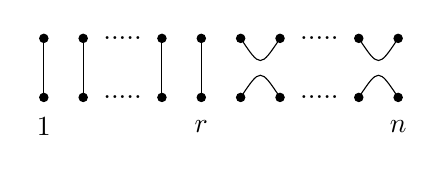
\begin{tikzpicture}
[scale=0.5,x=1cm, y=1.5cm]
\filldraw (0,0) circle (3pt); \filldraw (1,0) circle (3pt); \draw (2,0) node{.....};\filldraw (3,0) circle (3pt);\filldraw (4,0) circle (3pt);
\filldraw (5,0) circle (3pt); \filldraw (6,0) circle (3pt); \draw (7,0) node{.....};\filldraw (8,0) circle (3pt);\filldraw (9,0) circle (3pt);
\filldraw (0,1) circle (3pt); \filldraw (1,1) circle (3pt); \draw (2,1) node{.....};\filldraw (3,1) circle (3pt);\filldraw (4,1) circle (3pt);
\filldraw (5,1) circle (3pt); \filldraw (6,1) circle (3pt); \draw (7,1) node{.....};\filldraw (8,1) circle (3pt);\filldraw (9,1) circle (3pt);
\draw (0,0)--(0,1);\draw (1,0)--(1,1);\draw (3,0)--(3,1);\draw (4,0)--(4,1);
\draw (5,0) .. controls (5.5,0.5) and (5.5,0.5).. (6,0); \draw (8,0) .. controls (8.5,0.5) and (8.5,0.5).. (9,0);
\draw (5,1) .. controls (5.5,0.5) and (5.5,0.5).. (6,1); \draw (8,1) .. controls (8.5,0.5) and (8.5,0.5).. (9,1);
\draw (0,-0.5)node{$1$}; \draw(4,-0.5)node{$r$};\draw(9,-0.5)node{$n$};
\end{tikzpicture}
\caption{The rank $r$-projection $\ep_r$}\label{epr}
\end{figure}
The element $\zeta_r$ depicted in Fig.\ \ref{zetar}
\begin{figure}[h]
\centering
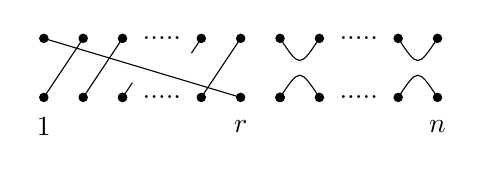
\begin{tikzpicture}
[scale=0.5,x=1cm,y=1.5cm]
\filldraw (0,0) circle (3pt); \filldraw (1,0) circle (3pt); \filldraw (2,0) circle (3pt);\draw (3,0) node{.....};\filldraw (4,0) circle (3pt);\filldraw (5,0) circle (3pt);
\filldraw (6,0) circle (3pt); \filldraw (6,0) circle (3pt); \draw (8,0) node{.....};\filldraw (6,0) circle (3pt);\filldraw (10,0) circle (3pt);
\filldraw (0,1) circle (3pt); \filldraw (1,1) circle (3pt); \filldraw (2,0) circle (3pt); \draw (3,1) node{.....};\filldraw (2,1) circle (3pt);\filldraw (5,1) circle (3pt); \filldraw (4,1) circle (3pt);\filldraw (7,0) circle (3pt);\filldraw (9,0) circle (3pt);
\filldraw (6,1) circle (3pt); \filldraw (7,1) circle (3pt); \draw (8,1) node{.....};\filldraw (9,1) circle (3pt);\filldraw (10,1) circle (3pt);
\draw (0,0)--(1,1);\draw (1,0)--(2,1);\draw (4,0)--(5,1);\draw (5,0)--(0,1);\draw (2,0)--(2.25,0.25); \draw (4,1)--(3.75,0.75);
\draw (6,0) .. controls (6.5,0.5) and (6.5,0.5).. (7,0); \draw (9,0) .. controls (9.5,0.5) and (9.5,0.5).. (10,0);
\draw (6,1) .. controls (6.5,0.5) and (6.5,0.5).. (7,1); \draw (9,1) .. controls (9.5,0.5) and (9.5,0.5).. (10,1);
\draw (0,-0.5)node{$1$}; \draw(5,-0.5)node{$r$};\draw(10,-0.5)node{$n$};
\end{tikzpicture}
\caption{The element $\zeta_r$}\label{zetar}
\end{figure}
is a generator of the group $\Hc$-class of $\ep_r$ in $\A_n$. But $\zeta_r$ is odd and therefore is definitely \textbf{not} contained in
$\mathfrak{EA}_n$. On the other hand, $\zeta_r^2$ is even and hence belongs to $\mathfrak{EA}_n$. It is easy to see that $\zeta_r^2$
generates a group of order $\frac{r}{2}$.
\end{proof}
Since the group of units of $\H(\A_n)$ is trivial we note that the subgroups of $\H(\A_n)$ are cyclic of order at most $\frac{n}{2}-1$.
Altogether we are able to detect a group in $\var\A_n$ that is not in $\var\H(\A_n)$:

\begin{Cor}
\label{differenceofanandhan} For each even number $n$ there exists a group in $\var\A_n$ that is not in $\var\H(\A_n)$.
\end{Cor}

\begin{proof} We have seen that all cyclic groups in $\var\H(\A_n)$
have even order less than $\frac n2$. On the other hand, each cyclic group of even order up to $n$ belongs to
$\var\A_n$. In order to find a (cyclic) group in $\var\A_n$ that is not in $\var\H(\A_n)$ it suffices to find an even
number $k\le n$ that does not divide the least common multiple of all even numbers less than $\frac n 2$. For such $k$
we may take the largest power of $2$ which is less than or equal to $n$.
\end{proof}

Since, for any $n$, all maximal subgroups of $\H(\A_n)$ have order at most $n-2$, by the same reasoning as in
Corollary~\ref{differenceofanandhan}, the next result is immediate.

\begin{Cor}
\label{differenceofanandhanodd} Let $n$ be a prime power; then the cyclic group of order $n$ belongs to $\var\A_n$ but
not to $\var\H(\A_n)$.
\end{Cor}

Finally, we show that the cases $n$ even or a prime power are the only ones for which there is a group in $\var\A_n$
that is not in $\var\H(\A_n)$. Therefore, our methods are applicable precisely in these cases.

\begin{figure}[ht]
\centering
\begin{picture}(100,100)(-10,5)
\gasset{AHnb=0,ExtNL=y,Nfill=y,Nw=1,Nh=1,Nmr=.5,NLdist=1} \node[NLangle=180](A1)(-5,10){$n$}
\node[NLangle=180](B1)(-5,20){$n-1$} \put(-5.5,28){$\vdots$} \node[NLangle=180](C1)(-5,40){$t+2$}
\node[NLangle=180](D1)(-5,50){$t+1$} \node[NLangle=180](E1)(-5,60){$t$} \node[NLangle=180](F1)(-5,70){$t-1$}
\put(-5.5,78){$\vdots$} \node[NLangle=180](G1)(-5,90){$2$} \node[NLangle=180](H1)(-5,100){$1$} \node(A2)(5,10){}
\node(B2)(5,20){} \put(4.5,28){$\vdots$} \node(C2)(5,40){} \node(D2)(5,50){} \node(E2)(5,60){} \node(F2)(5,70){}
\put(4.5,78){$\vdots$} \node(G2)(5,90){} \node(H2)(5,100){} \drawedge[curvedepth=-2](A1,B1){}
\drawedge[curvedepth=2](A2,B2){} \drawedge[curvedepth=-2](C1,D1){} \drawedge[curvedepth=2](C2,D2){}
\drawedge[curvedepth=2](E2,D2){} \drawedge[linegray=1,ELside=r](A1,A2){$\varepsilon_{t+1}$} \drawedge(E1,E2){}
\drawedge(F1,F2){} \drawedge(G1,G2){} \drawedge(H1,H2){} \node(A3)(15,10){} \node(B3)(15,20){} \put(14.5,28){$\vdots$}
\node(C3)(15,40){} \node(D3)(15,50){} \node(E3)(15,60){} \node(F3)(15,70){} \put(14.5,78){$\vdots$} \node(G3)(15,90){}
\node(H3)(15,100){} \drawedge[curvedepth=2](A3,B3){} \drawedge[curvedepth=-2](A2,B2){} \drawedge[curvedepth=2](D3,E3){}
\drawedge[curvedepth=-2](E3,F3){} \drawedge[linegray=1,ELside=r](A2,A3){$\varepsilon_{t}$} \drawedge(C3,C2){}
\drawedge(F3,F2){} \drawedge(G3,G2){} \drawedge(H3,H2){} \node(A3)(15,10){} \node(B3)(15,20){} \put(14.5,28){$\vdots$}
\node(C3)(15,40){} \node(D3)(15,50){} \node(E3)(15,60){} \node(F3)(15,70){} \put(14.5,78){$\vdots$} \node(G3)(15,90){}
\node(H3)(15,100){} \drawedge[curvedepth=2](A3,B3){} \drawedge[curvedepth=-2](A2,B2){} \drawedge[curvedepth=2](D3,E3){}
\drawedge[curvedepth=-2](E3,F3){} \drawedge[linegray=1,ELside=r](A2,A3){$\varepsilon_{t}$} \node(A4)(25,10){}
\node(B4)(25,20){} \put(24.5,28){$\vdots$} \node(C4)(25,40){} \node(D4)(25,50){} \node(E4)(25,60){} \node(F4)(25,70){}
\put(24.5,78){$\vdots$} \node(G4)(25,90){} \node(H4)(25,100){} \drawedge[curvedepth=-2](A3,B3){}
\drawedge[curvedepth=2](A4,B4){} \drawedge[curvedepth=2](E4,F4){}
\drawedge[linegray=1,ELside=r](A3,A4){$\varepsilon_{t-1}$} \drawedge(C3,C4){} \drawedge(D3,D4){} \drawedge(G3,G4){}
\drawedge(H3,H4){} \put(29,10){$\dots$} \put(29,20){$\dots$} \put(29,40){$\dots$} \put(29,50){$\dots$}
\put(29,60){$\dots$} \put(29,90){$\dots$} \put(29,100){$\dots$} \node(A5)(37,10){} \node(B5)(37,20){}
\put(36.5,28){$\vdots$} \node(C5)(37,40){} \node(D5)(37,50){} \node(E5)(37,60){} \put(36.5,68){$\vdots$}
\node(F5)(37,80){} \node(G5)(37,90){} \node(H5)(37,100){} \drawedge[curvedepth=2](G5,F5){} \node(A6)(47,10){}
\node(B6)(47,20){} \put(46.5,28){$\vdots$} \node(C6)(47,40){} \node(D6)(47,50){} \node(E6)(47,60){}
\put(46.5,68){$\vdots$} \node(F6)(47,80){} \node(G6)(47,90){} \node(H6)(47,100){} \drawedge[curvedepth=-2](G6,F6){}
\drawedge[curvedepth=-2](G6,H6){} \drawedge[curvedepth=-2](A5,B5){} \drawedge[curvedepth=2](A6,B6){}
\drawedge[linegray=1,ELside=r](A5,A6){$\varepsilon_2$} \drawedge(C5,C6){} \drawedge(D5,D6){} \drawedge(E5,E6){}
\drawedge(H5,H6){} \node(A7)(57,10){} \node(B7)(57,20){} \put(56.5,28){$\vdots$} \node(C7)(57,40){} \node(D7)(57,50){}
\node(E7)(57,60){} \put(56.5,68){$\vdots$} \node(F7)(57,80){} \node(G7)(57,90){} \node(H7)(57,100){}
\drawedge[curvedepth=2](G7,H7){} \drawedge[curvedepth=-2](A6,B6){} \drawedge[curvedepth=2](A7,B7){}
\drawedge[curvedepth=-2](A7,B7){} \drawedge[linegray=1,ELside=r](A6,A7){$\varepsilon_1$} \drawedge(C7,C6){}
\drawedge(D7,D6){} \drawedge(E7,E6){} \drawedge(F6,F7){} \drawbcedge(H7,67,130,C7,67,10){} \node(A8)(77,10){}
\node(B8)(77,20){} \put(76.5,28){$\vdots$} \node(C8)(77,40){} \node(D8)(77,50){} \node(E8)(77,60){}
\put(76.5,68){$\vdots$} \node(F8)(77,80){} \node(G8)(77,90){} \node(H8)(77,100){} \drawedge[curvedepth=2](A8,B8){}
\drawedge[curvedepth=-2](A8,B8){} \drawedge[linegray=1,ELside=r](A7,A8){$\varepsilon_0$} \drawedge(D7,D8){}
\drawedge(E7,E8){} \drawedge(F7,F8){} \drawedge(G7,G8){} \drawbcedge(C8,67,10,H8,67,130){} \node(A9)(87,10){}
\node(B9)(87,20){} \put(86.5,28){$\vdots$} \node(C9)(87,40){} \node(D9)(87,50){} \node(E9)(87,60){}
\put(86.5,68){$\vdots$} \node(F9)(87,80){} \node(G9)(87,90){} \node(H9)(87,100){} \drawedge[curvedepth=2](A9,B9){}
\drawedge[linegray=1,ELside=r](A8,A9){$\varepsilon_{t+1}$} \drawedge[curvedepth=-2](C8,D8){}
\drawedge[curvedepth=2](C9,D9){} \drawedge(E9,E8){} \drawedge(F9,F8){} \drawedge(G9,G8){} \drawedge(H9,H8){}
\end{picture}
\caption{A cycle of order $t$ as a product of projections in $\A_n$}\label{shortdecomposition}
\end{figure}

\begin{Prop}
\label{noprimepowerodd} If $n$ is odd and not a prime power then the groups in $\var\A_n$ and $\var\H(\A_n)$ are the
same.
\end{Prop}
\begin{proof} Every element of $\A_n$ has odd rank. Let $t<n$ be odd.
We define projections $\ep_0,\ep_1,\dots,\ep_{t+1}$ as follows. Each $\ep_i$, $i=0,1,\dots,t+1$, has the outer strings
$\{t+3,t+4\},\dots,\{n-1,n\}$ and the corresponding inner strings; besides those, the projection $\ep_0$ has the outer
string $\{1,t+2\}$ and the inner string $\{1',(t+2)'\}$ and each of the projections $\ep_i$, $i=1,\dots,t+1$, has the
outer string $\{i,i+1\}$ and the outer string $\{i',(i+1)'\}$. Finally, all remaining elements of $\wt{[n]}$ are
involved in the through strings  $\{k,k'\}$.

One then readily verifies (see Fig.\,\ref{shortdecomposition}) that $\al=\ep_{t+1}\ep_t\cdots \ep_0\ep_{t+1}$ has the
same inner and outer strings as $\ep_{t+1}$ hence $\al\mathrel{\Hc}\ep_{t+1}$. Moreover, the through strings of $\al$
are
$$\{1,3'\},\{2,4'\},\dots,\{t-1,1'\},\{t,2'\}.$$
Via \eqref{embeddingofSk}, $\al$ realizes the cyclic permutation $k\mapsto k+2\!\pmod{t}$ which has order $t$ since $t$
is odd. Thus, for each odd $t<n$, the semigroup $\H(\A_n)$ contains a cyclic group of order $t$ as an involutory subsemigroup.
The maximal subgroups of $\A_n$ are precisely the cyclic groups of odd order at most $n$. So, we have already shown
that $\var\H(\A_n)$ contains each maximal subgroup of $\A_n$, with the possible exception of the group of units of
$\A_n$ which is cyclic of order $n$. Since $n$ is not a prime power, $n=k\ell$ for some co-prime numbers $k,\ell$. As
already pointed out, the cyclic groups $\mathcal{C}_k$ and $\mathcal{C}_\ell$ of orders $k$ and $\ell$, respectively,
belong to $\var\H(\A_n)$ whence so does the cyclic group of order $n$ which is isomorphic to $\mathcal{C}_k
\times\mathcal{C}_\ell$.
\end{proof}
\begin{Cor} There exists a group in $\var\A_n$ that is not in
$\var\H(\A_n)$ if and only if $n$ is even or a prime power.
\end{Cor}

We can also characterize the even numbers $n$ for which there exists a group in $\var\mathfrak{EA}_n$ which is not in
$\var\H(\mathfrak{EA}_n)$. Indeed, it was shown in \cite{complexity} that for even $n$---recall that $\mathfrak{EA}_n$ is only defined for
even $n$---, the semigroup $\H(\A_n)=\H(\mathfrak{EA}_n)$ consists of the identity element $1$ together with all elements of
$\mathfrak{EA}_n$ whose rank is strictly smaller than $n$. It follows that the maximal subgroups of $\mathfrak{EA}_n$ are the cyclic groups
of orders $\frac n2, \frac n2 -1,\dots, 1$ while the maximal subgroups of $\H(\mathfrak{EA}_n)$ are the cyclic groups of orders $\frac n2
-1,\frac n2-2,\dots,1$. This shows the next result.
\begin{Cor}
Let $n$ be even; then there exists a group in $\var\mathfrak{EA}_n$ which is not in $\var\H(\mathfrak{EA}_n)$ if and only if $\frac n2$ is
a prime power.
\end{Cor}

In contrast to the ordinary annular case, it is no longer true that there is a group in $\var P\A_n$ that is not in $\var\H(P\A_n)$ for
each even $n$. The fact that some elements of $\wt{[n]}$ need not be involved in any string gives the projections more freedom to gain
cyclic permutations in $\H(P\A_n)$, as the following result demonstrates.

\begin{Prop}
\label{partialannular} For each $n\ge 5$ and $t\le n-3$ there exists a cyclic subgroup of order $t$ in $\H(P\A_n)$.
\end{Prop}

\begin{proof}
For odd $t$ this follows immediately from Proposition \ref{noprimepowerodd}. For even $t$ it can be shown that the
element $\al$ consisting of the through strings
$$\{1,2'\}, \{2,3'\},\dots,\{t-1,t'\},\{t,1'\}$$
along with the outer string $\{t{+}2,t{+}3\}$ and the inner string $\{(t{+}2)',(t{+}3)'\}$, and else having no other
strings can be written as a product of $\frac{5t}2 + 4$ projections, see Fig.\,\ref{longdecomposition}. Clearly, $\al$
realizes a cyclic permutation of order~$t$.
\end{proof}

\begin{figure}[p]
\centering \unitlength=.775mm {\small
\begin{picture}(100,235)(-100,-52)
\begin{rotate}{90}
\gasset{AHnb=0,ExtNL=y,Nfill=y,Nw=1,Nh=1,Nmr=.5,NLdist=1} \node[NLangle=180](A1)(-45,0){$t+3$}
\node[NLangle=180](B1)(-45,10){$t+2$} \node[NLangle=180](C1)(-45,20){$t+1$} \node[NLangle=180](D1)(-45,30){$t$}
\node[NLangle=180](E1)(-45,40){$t-1$} \node[NLangle=180](F1)(-45,50){$t-2$} \node[NLangle=180](G1)(-45,80){$3$}
\node[NLangle=180](H1)(-45,90){$2$} \node[NLangle=180](I1)(-45,100){$1$} \node(A2)(-35,0){} \node(B2)(-35,10){}
\node(C2)(-35,20){} \node(D2)(-35,30){} \node(E2)(-35,40){} \node(F2)(-35,50){} \node(G2)(-35,80){} \node(H2)(-35,90){}
\node(I2)(-35,100){} \drawedge[curvedepth=-2](A1,B1){} \drawedge[curvedepth=2](A2,B2){} \drawedge(D1,D2){}
\drawedge(E1,E2){} \drawedge(F1,F2){} \drawedge(G1,G2){} \drawedge(H1,H2){} \drawedge(I1,I2){}
\drawedge[linegray=1,ELside=r](A1,A2){$\varepsilon_1$} \drawedge[curvedepth=-3](B2,D2){} \put(-46,65){$\vdots$}
\put(-36,65){$\vdots$} \put(-26,65){$\vdots$} \put(-16,65){$\vdots$} \put(-6,65){$\vdots$} \put(4,65){$\vdots$}
\node(A3)(-25,0){} \node(B3)(-25,10){} \node(C3)(-25,20){} \node(D3)(-25,30){} \node(E3)(-25,40){} \node(F3)(-25,50){}
\node(G3)(-25,80){} \node(H3)(-25,90){} \node(I3)(-25,100){} \drawedge[curvedepth=3](B3,D3){}
\drawedge[curvedepth=-2](D3,E3){} \drawedge(A3,A2){$\varepsilon_2$} \drawedge(E3,E2){} \drawedge(F3,F2){}
\drawedge(G3,G2){} \drawedge(H3,H2){} \drawedge(I3,I2){} \node(A4)(-15,0){} \node(B4)(-15,10){} \node(C4)(-15,20){}
\node(D4)(-15,30){} \node(E4)(-15,40){} \node(F4)(-15,50){} \node(G4)(-15,80){} \node(H4)(-15,90){}
\node(I4)(-15,100){} \drawedge[curvedepth=2](D4,E4){} \drawedge[curvedepth=2](D4,C4){}
\drawedge[ELside=r](A3,A4){$\varepsilon_3$} \drawedge(B3,B4){} \drawedge(F3,F4){} \drawedge(G3,G4){} \drawedge(H3,H4){}
\drawedge(I3,I4){} \node(A5)(-5,0){} \node(B5)(-5,10){} \node(C5)(-5,20){} \node(D5)(-5,30){} \node(E5)(-5,40){}
\node(F5)(-5,50){} \node(G5)(-5,80){} \node(H5)(-5,90){} \node(I5)(-5,100){} \drawedge[curvedepth=3](F5,D5){}
\drawedge[curvedepth=-2](D5,C5){} \drawedge(A5,A4){$\varepsilon_4$} \drawedge(B5,B4){} \drawedge(F5,F4){}
\drawedge(G5,G4){} \drawedge(H5,H4){} \drawedge(I5,I4){} \node(A6)(5,0){} \node(B6)(5,10){} \node(C6)(5,20){}
\node(D6)(5,30){} \node(E6)(5,40){} \node(F6)(5,50){} \node(G6)(5,80){} \node(H6)(5,90){} \node(I6)(5,100){}
\drawedge[curvedepth=-3](F6,D6){} \drawedge[ELside=r](A5,A6){$\varepsilon_5$} \drawedge(B5,B6){} \drawedge(C5,C6){}
\drawedge(G5,G6){} \drawedge(H5,H6){} \drawedge(I5,I6){} \put(9,0){$\dots$} \put(9,10){$\dots$} \put(9,20){$\dots$}
\put(9,30){$\dots$} \put(9,80){$\dots$} \put(9,90){$\dots$} \put(9,100){$\dots$} \node(A7)(17,0){} \node(B7)(17,10){}
\node(C7)(17,20){} \node(D7)(17,30){} \node(E7)(17,60){} \node(F7)(17,70){} \node(G7)(17,80){} \node(H7)(17,90){}
\node(I7)(17,100){} \drawedge[curvedepth=-2](F7,G7){} \node(A8)(27,0){} \node(B8)(27,10){} \node(C8)(27,20){}
\node(D8)(27,30){} \node(E8)(27,60){} \node(F8)(27,70){} \node(G8)(27,80){} \node(H8)(27,90){} \node(I8)(27,100){}
\put(16,45){$\vdots$} \put(26,45){$\vdots$} \put(36,45){$\vdots$} \put(46,45){$\vdots$} \put(56,45){$\vdots$}
\put(66,45){$\vdots$} \put(86,45){$\vdots$} \put(96,45){$\vdots$} \put(106,45){$\vdots$} \put(116,45){$\vdots$}
\put(126,45){$\vdots$} \drawedge(H7,H8){} \drawedge(I7,I8){} \drawedge(D7,D8){} \drawedge(C7,C8){} \drawedge(B7,B8){}
\drawedge(A7,A8){} \drawedge[curvedepth=2](F8,G8){} \drawedge[curvedepth=2](F8,E8){} \node(A9)(37,0){}
\node(B9)(37,10){} \node(C9)(37,20){} \node(D9)(37,30){} \node(E9)(37,60){} \node(F9)(37,70){} \node(G9)(37,80){}
\node(H9)(37,90){} \node(I9)(37,100){} \drawedge(I9,I8){} \drawedge(H9,H8){} \drawedge(D9,D8){} \drawedge(C9,C8){}
\drawedge(B9,B8){} \drawedge(A9,A8){} \drawedge[curvedepth=-2](F9,E9){} \drawedge[curvedepth=-3](F9,H9){}
\node(A10)(47,0){} \node(B10)(47,10){} \node(C10)(47,20){} \node(D10)(47,30){} \node(E10)(47,60){} \node(F10)(47,70){}
\node(G10)(47,80){} \node(H10)(47,90){} \node(I10)(47,100){} \drawedge(I9,I10){} \drawedge(E9,E10){}
\drawedge(D9,D10){} \drawedge(C9,C10){} \drawedge(B9,B10){} \drawedge(A9,A10){} \drawedge[curvedepth=3](F10,H10){}
\drawedge[curvedepth=-2](H10,I10){} \node(A11)(57,0){} \node(B11)(57,10){} \node(C11)(57,20){} \node(D11)(57,30){}
\node(E11)(57,60){} \node(F11)(57,70){} \node(G11)(57,80){} \node(H11)(57,90){} \node(I11)(57,100){}
\drawedge(F11,F10){} \drawedge(E11,E10){} \drawedge(D11,D10){} \drawedge(C11,C10){} \drawedge(B11,B10){}
\drawedge(A11,A10){$\varepsilon_{\frac{3t}2}$} \drawedge[curvedepth=2](H11,I11){} \drawedge[curvedepth=3](I11,G11){}
\node(A12)(67,0){} \node(B12)(67,10){} \node(C12)(67,20){} \node(D12)(67,30){} \node(E12)(67,60){} \node(F12)(67,70){}
\node(G12)(67,80){} \node(H12)(67,90){} \node(I12)(67,100){} \drawedge(F11,F12){} \drawedge(E11,E12){}
\drawedge(D11,D12){} \drawedge(C11,C12){} \drawedge(B11,B12){} \drawedge(A12,A11){$\varepsilon_{\frac{3t}2+1}$}
\drawedge[curvedepth=-3](I12,G12){} \drawbcedge(I12,77,130,A12,77,-30){} \node(A13)(87,0){} \node(B13)(87,10){}
\node(C13)(87,20){} \node(D13)(87,30){} \node(E13)(87,60){} \node(F13)(87,70){} \node(G13)(87,80){} \node(H13)(87,90){}
\node(I13)(87,100){} \drawbcedge(I13,77,130,A13,77,-30){} \drawedge[curvedepth=-2](H13,I13){} \drawedge(G13,G12){}
\drawedge(F13,F12){} \drawedge(E13,E12){} \drawedge(D13,D12){} \drawedge(C13,C12){} \drawedge(B13,B12){}
\drawedge[linegray=1](A13,A12){$\varepsilon_{\frac{3t}2+2}$} \node(A14)(97,0){} \node(B14)(97,10){} \node(C14)(97,20){}
\node(D14)(97,30){} \node(E14)(97,60){} \node(F14)(97,70){} \node(G14)(97,80){} \node(H14)(97,90){}
\node(I14)(97,100){} \drawedge[curvedepth=2](H14,I14){} \drawedge[curvedepth=2](H14,G14){} \drawedge(G13,G14){}
\drawedge(F13,F14){} \drawedge(E13,E14){} \drawedge(D13,D14){} \drawedge(C13,C14){} \drawedge(B13,B14){}
\drawedge[linegray=1](A14,A13){$\varepsilon_{\frac{3t}2+3}$} \node(A15)(107,0){} \node(B15)(107,10){}
\node(C15)(107,20){} \node(D15)(107,30){} \node(E15)(107,60){} \node(F15)(107,70){} \node(G15)(107,80){}
\node(H15)(107,90){} \node(I15)(107,100){} \drawedge(I15,I14){} \drawedge(F15,F14){} \drawedge(E15,E14){}
\drawedge(D15,D14){} \drawedge(C15,C14){} \drawedge(B15,B14){} \drawedge[curvedepth=2](G15,F15){}
\drawedge[curvedepth=-2](H15,G15){} \drawedge[linegray=1](A15,A14){$\varepsilon_{\frac{3t}2+4}$} \node(A16)(117,0){}
\node(B16)(117,10){} \node(C16)(117,20){} \node(D16)(117,30){} \node(E16)(117,60){} \node(F16)(117,70){}
\node(G16)(117,80){} \node(H16)(117,90){} \node(I16)(117,100){} \drawedge(I15,I16){} \drawedge(H15,H16){}
\drawedge(E15,E16){} \drawedge(D15,D16){} \drawedge(C15,C16){} \drawedge(B15,B16){} \drawedge[curvedepth=-2](G16,F16){}
\drawedge[curvedepth=2](F16,E16){} \node(A17)(127,0){} \node(B17)(127,10){} \node(C17)(127,20){} \node(D17)(127,30){}
\node(E17)(127,60){} \node(F17)(127,70){} \node(G17)(127,80){} \node(H17)(127,90){} \node(I17)(127,100){}
\drawedge(I17,I16){} \drawedge(H17,H16){} \drawedge(G17,G16){} \drawedge(D17,D16){} \drawedge(C17,C16){}
\drawedge(B17,B16){} \drawedge[curvedepth=-2](F17,E17){} \put(131,0){$\dots$} \put(131,10){$\dots$}
\put(131,20){$\dots$} \put(131,30){$\dots$} \put(131,70){$\dots$} \put(131,80){$\dots$} \put(131,90){$\dots$}
\put(131,100){$\dots$} \node(A18)(139,0){} \node(B18)(139,10){} \node(C18)(139,20){} \node(D18)(139,30){}
\node(E18)(139,40){} \node(F18)(139,70){} \node(G18)(139,80){} \node(H18)(139,90){} \node(I18)(139,100){}
\drawedge[curvedepth=-2](D18,E18){} \put(138,55){$\vdots$} \put(148,55){$\vdots$} \put(158,55){$\vdots$}
\put(168,55){$\vdots$} \put(178,55){$\vdots$} \node(A19)(149,0){} \node(B19)(149,10){} \node(C19)(149,20){}
\node(D19)(149,30){} \node(E19)(149,40){} \node(F19)(149,70){} \node(G19)(149,80){} \node(H19)(149,90){}
\node(I19)(149,100){} \drawedge(I18,I19){} \drawedge(H18,H19){} \drawedge(G18,G19){} \drawedge(F18,F19){}
\drawedge(C18,C19){} \drawedge(B18,B19){} \drawedge[curvedepth=2](D19,C19){} \drawedge[curvedepth=2](D19,E19){}
\drawedge[linegray=1](A19,A18){$\varepsilon_{\frac{5t}2+1}$} \node(A20)(159,0){} \node(B20)(159,10){}
\node(C20)(159,20){} \node(D20)(159,30){} \node(E20)(159,40){} \node(F20)(159,70){} \node(G20)(159,80){}
\node(H20)(159,90){} \node(I20)(159,100){} \drawedge(I20,I19){} \drawedge(H20,H19){} \drawedge(G20,G19){}
\drawedge(F20,F19){} \drawedge(E20,E19){} \drawedge(B20,B19){} \drawedge[curvedepth=-2](D20,C20){}
\drawedge[curvedepth=-2](B20,C20){} \drawedge[linegray=1](A20,A19){$\varepsilon_{\frac{5t}2+2}$} \node(A21)(169,0){}
\node(B21)(169,10){} \node(C21)(169,20){} \node(D21)(169,30){} \node(E21)(169,40){} \node(F21)(169,70){}
\node(G21)(169,80){} \node(H21)(169,90){} \node(I21)(169,100){} \drawedge(I20,I21){} \drawedge(H20,H21){}
\drawedge(G20,G21){} \drawedge(F20,F21){} \drawedge(E20,E21){} \drawedge(D20,D21){} \drawedge[curvedepth=-2](A21,B21){}
\drawedge[curvedepth=2](B21,C21){} \drawedge[linegray=1](A21,A20){$\varepsilon_{\frac{5t}2+3}$} \node(A22)(179,0){}
\node(B22)(179,10){} \node(C22)(179,20){} \node(D22)(179,30){} \node(E22)(179,40){} \node(F22)(179,70){}
\node(G22)(179,80){} \node(H22)(179,90){} \node(I22)(179,100){} \drawedge(I22,I21){} \drawedge(H22,H21){}
\drawedge(G22,G21){} \drawedge(F22,F21){} \drawedge(E22,E21){} \drawedge(D22,D21){} \drawedge[curvedepth=2](A22,B22){}
\drawedge[linegray=1](A22,A21){$\varepsilon_{\frac{5t}2+4}$}
\end{rotate}
\end{picture}}
\caption{A cycle of order $t$ as a product of projections in $P\A_n$}\label{longdecomposition}
\end{figure}

From this we obtain:
\begin{Cor}
\label{partialannularbadcases} If $n\notin\{p^k,p^k+1,2^k+2\}$ for each prime $p$ and each $k\ge 1$, then
$\var\H(P\A_n)$ and $\var P\A_n$ contain the same groups.
\end{Cor}
\begin{proof} We may assume that $n\ge 15$. As already mentioned,
the variety of all groups in $\var P\A_n$ is generated by all cyclic groups of orders at most $n$. By
Proposition~\ref{partialannular}, all cyclic groups of orders at most $n-3$ belong to $\var\H(P\A_n)$. Since $n$ is not
a prime power it can be factored as $n=k\ell$ with $k,\ell$ co-prime and $k,\ell\le n-3$. Since the cyclic groups of
order $k$ and $\ell$ belong to $\var\H(P\A_n)$, so does the cyclic group of order $n$. The same reasoning applies to
the cyclic group of order $n-1$. Consider finally the case of $n-2$. By assumption, $n-2$ either is an odd prime power
or has at least two distinct prime factors. In the former case the claim follows from the proof of
Proposition~\ref{noprimepowerodd} and in the latter case the argument is the same as for $n$ and $n-1$.
\end{proof}

On the other hand, the converse of Corollary~\ref{partialannularbadcases} also holds.

\begin{Prop}
\label{partialannulargoodcases} If $n\in\{p^k,p^k+1,2^k+2\}$ for some prime $p$ and some positive integer $k$, then
there exists a group in $\var P\A_n$ which is not in $\var\H(P\A_n)$.
\end{Prop}

\begin{proof} The case $n=p^k$ is obvious. Since the product of any two
\emph{distinct} projections of rank $n-1$ has rank less than $n-1$, the group $\Hc$-class in $\H(P\A_n)$ of any
projection of rank $n-1$ is trivial, implying the claim for the case $n=p^k+1$.

Finally, in case $n=2^k+2$ we show that the cyclic group of order $2^k=n-2$ is not in $\var\H(P\A_n)$. Let $\ep$ be a
projection of rank $n-2$ containing the outer string $\{i,i+1\}$ and the inner string $\{i',(i+1)'\}$ and let
$\ep^\circ$ be the projection obtained from $\ep$ by removing these two strings. If $\eta$ is a projection of rank
$n-1$ such that $\eta\ep$ has rank $n-2$, then $\eta\ep=\ep^\circ\ep$ (and likewise $\ep\eta=\ep\ep^\circ$). Hence, if
$\al$ is {a product of projections and of rank $n-2$} then we may assume that all these projections have rank  $n-2$.
Moreover, any product of two distinct projections of rank $n-2$ that have only through strings has rank less than
$n-2$. Finally, let $\ep_1, \ep_2, \ep_3$ be projections of rank $n-2$ such that $\ep_1$ and $\ep_3$ have outer and
inner strings but $\ep_2$ does not. If $\ep_1\ep_2\ep_3$ has rank $n-2$ then $\ep_1=\ep_3$ and
$\ep_1\ep_2\ep_3=\ep_1\ep_3=\ep_1$.

Let $\alpha$ be of rank $n-2$ and assume that it is a product of projections: $\alpha=\ep_0\ep_1\cdots \ep_r$. The
observations in the preceding paragraph imply that in addition we may assume that $\ep_i$ has rank $n-2$ for each
$i=0,\dots,r$ and that $\ep_1,\dots, \ep_{r-1}$ have inner and outer strings, that is, $\ep_1,\dots, \ep_{r-1}$ belong
to $\A_n$. Assume further that $\alpha$ is contained in a subgroup of $\H (P\A_n)$. We intend to prove that the order
of $\alpha$ is at most $\frac{n-2}2=2^{k-1}$. For this purpose we may assume that $\alpha$ is $\Hc$-related to a
projection $\ep$. This implies immediately that $\ep_0=\ep=\ep_r$.

Now consider two cases: (i) $\ep$ has an inner and an outer string, that is, $\ep$ belongs to $\A_n$, and (ii) $\ep$
has only through strings, that is, $\ep$ does not belong to $\A_n$. In the first case, $\alpha$ belongs to $\H(\A_n)$
and so the order of $\alpha$ is at most $\frac{n-2}2$ by Lemma \ref{subgroupsofDr}.

In the second case, we get $\ep_1=\ep_{r-1}$ and $\ep=\ep_1^\circ$ since $\ep\ep_1$ as well as $\ep_{r-1}\ep$ have
rank $n-2$. From this it follows that the set $\{\ep,\ep_1,\ep\ep_1,\ep_1\ep\}$ forms a $2\times 2$-rectangular band
under multiplication. In particular, $\ep$ and $\ep_1$ are $\Dc$-related in $\H (P\A_n)$. Green's Lemma implies that
the order of $\alpha$ is the same as the order of $\ep_1\alpha\ep_1=\ep_1\cdots\ep_{r-1}$. The latter element belongs
to $\H(\A_n)$, so its order is at most $\frac{n-2}2$, again by Lemma \ref{subgroupsofDr}. Since no group element
of rank less than $n-2$ can have order $n-2$ we actually have shown that $\H (P\A_n)$ does not contain a group element
of order $n-2=2^k$.

Altogether, the cyclic group of order $2^k$ belongs to $\var P\A_n$ but not to $\var\H (P\A_n)$, just as required.
\end{proof}
Having thus completely examined when condition (i) mentioned in the introduction to Section \ref{inverse involution} is
fulfilled we turn to condition (ii).

\subsubsection{Membership of $\mathcal{K}_3$}

In order to complete the results which make an application of Theorem \ref{Theorem 2.1} possible, we need to check
membership of $\mathcal{K}_3$.

\begin{Prop}\label{membershipofC3}
The regular $^*$-semigroup $\mathcal{K}_3$ is contained in
\begin{enumerate}
\item $\var\C_n$ for each $n\ge 2$,
\item $\var P\A_n\subseteq \var P\B_n$ for each $n\ge 3$,
\item $\var \A_n\subseteq \var \B_n$ for each $n\ge 4$ and $\var\mathfrak{EA}_n$ for each even $n\ge 4$.
\end{enumerate}
\end{Prop}
\begin{proof} In the first case, consider the regular $^*$-subsemigroup $\mathcal{U}_1$ of $\C_2$
generated by the projections of rank~1---these are
\[
\{\{1,1',2,2'\}\},\{\{1,1'\},\{2\},\{2'\}\}, \{\{1\},\{1'\},\{2,2'\}\}.
\]
It is easy to calculate that $\mathcal{U}_1$ contains 13 partitions: 9 of rank~1 and 4 of rank~0. The $\Dc$-class of $\mathcal{U}_1$
consisting of the partitions of rank~1 is shown in Fig.\,\ref{C3inC2} where the idempotents are marked with $\star$.
\begin{figure}[ht]
\centering
\begin{picture}(50,50)
\multiput(0,0)(0,20){3}{%
\multiput(0,0)(20,0){3}{\put(0,0){$\bullet$}%
\put(0,8){$\bullet$}\put(8,0){$\bullet$}\put(8,8){$\bullet$}}} \drawrect(-1,39,11,51) \multiput(4,4)(0,20){3}{$\star$}
\multiput(24,24)(0,20){2}{$\star$} \multiput(44,4)(0,40){2}{$\star$}
\multiput(0,0)(20,0){3}{%
\drawrect(-1,19,3,23)} \drawline[AHnb=0](-1,27)(-1,31)(11,31)(11,19)(7,19)(7,27)(-1,27)
\multiput(0,0)(20,0){3}{%
\drawrect(-1,7,3,11)} \drawline[AHnb=0](-1,-1)(-1,3)(7,3)(7,11)(11,11)(11,-1)(-1,-1)
\multiput(28,-8)(0,20){3}{%
\drawrect(-1,7,3,11)}
\multiput(48,0)(0,20){3}{%
\drawrect(-1,7,3,11)} \drawrect(19,27,31,31) \drawrect(39,-1,51,3)
\drawline[AHnb=0](19,39)(19,51)(31,51)(31,47)(23,47)(23,39)(19,39)
\drawline[AHnb=0](39,39)(39,51)(43,51)(43,43)(51,43)(51,39)(39,39) \drawline[AHnb=0](21,-2)(18,1)(29,12)(32,9)(21,-2)
\drawline[AHnb=0](38,29)(41,32)(52,21)(49,18)(38,29)
\end{picture}
\caption{The upper $\Dc$-class of the subsemigroup $\mathcal{U}_1$ of $\C_2$}\label{C3inC2}
\end{figure}

Now it is clear that if one factors $\mathcal{U}_1$ by the ideal of all elements of rank~0, then the resulting regular
$^*$-semigroup is isomorphic to $\mathcal{K}_3$. Thus, $\mathcal{K}_3$ belongs to the variety $\var\C_2$, and hence, to
the variety $\var\C_n$ for each $n\ge 2$.

For the second case consider the involutory subsemigroup $\mathcal{U}_2$ of $P\A_3$ generated by the projections
\begin{gather*}
\{\{1,1'\},\{2,3\},\{2',3'\}\},\\
\{\{1,2\},\{1',2'\},\{3,3'\}\},\\
\{\{1,1'\},\{2\},\{2'\},\{3\},\{3'\}\}.
\end{gather*}
Again it is easy to calculate that $\mathcal{U}_2$ contains 9 partitions of rank~1 and 9~partitions of rank~0. The
partitions of rank~1 form a regular $\Dc$-class depicted in Fig.\,\ref{C3inPA3}. As above, the idempotents are marked
with $\star$.
\begin{figure}[hb]
\centering \unitlength 1.25mm
\begin{picture}(40,40)
\gasset{AHnb=0,ExtNL=y,Nfill=y,Nw=1,Nh=1,Nmr=.5,NLdist=1} \multiput(3,3)(0,16){3}{$\star$}
\multiput(19,19)(0,16){2}{$\star$} \multiput(35,3)(0,32){2}{$\star$} \node(A11)(0,0){} \node(A12)(0,4){}
\node(A13)(0,8){} \node(B11)(8,0){} \node(B12)(8,4){} \node(B13)(8,8){} \drawedge(A13,B13){}
\drawedge[curvedepth=2](B11,B12){} \node(A14)(0,16){} \node(A15)(0,20){} \node(A16)(0,24){} \node(B14)(8,16){}
\node(B15)(8,20){} \node(B16)(8,24){} \drawedge[curvedepth=2](B14,B15){} \drawedge[curvedepth=2](A16,A15){}
\drawedge(A14,B16){} \node(A17)(0,32){} \node(A18)(0,36){} \node(A19)(0,40){} \node(B17)(8,32){} \node(B18)(8,36){}
\node(B19)(8,40){} \drawedge[curvedepth=2](B17,B18){} \drawedge[curvedepth=2](A18,A17){} \drawedge(A19,B19){}
\node(A21)(16,0){} \node(A22)(16,4){} \node(A23)(16,8){} \node(B21)(24,0){} \node(B22)(24,4){} \node(B23)(24,8){}
\drawedge(A23,B21){} \drawedge[curvedepth=2](B22,B23){} \node(A24)(16,16){} \node(A25)(16,20){} \node(A26)(16,24){}
\node(B24)(24,16){} \node(B25)(24,20){} \node(B26)(24,24){} \drawedge(A24,B24){} \drawedge[curvedepth=2](B25,B26){}
\drawedge[curvedepth=2](A26,A25){} \node(A27)(16,32){} \node(A28)(16,36){} \node(A29)(16,40){} \node(B27)(24,32){}
\node(B28)(24,36){} \node(B29)(24,40){} \drawedge(A29,B27){} \drawedge[curvedepth=2](B28,B29){}
\drawedge[curvedepth=2](A28,A27){} \node(A31)(32,0){} \node(A32)(32,4){} \node(A33)(32,8){} \node(B31)(40,0){}
\node(B32)(40,4){} \node(B33)(40,8){} \drawedge(A33,B33){} \node(A34)(32,16){} \node(A35)(32,20){} \node(A36)(32,24){}
\node(B34)(40,16){} \node(B35)(40,20){} \node(B36)(40,24){} \drawedge(A34,B36){} \drawedge[curvedepth=2](A36,A35){}
\node(A37)(32,32){} \node(A38)(32,36){} \node(A39)(32,40){} \node(B37)(40,32){} \node(B38)(40,36){} \node(B39)(40,40){}
\drawedge(A39,B39){} \drawedge[curvedepth=2](A38,A37){}
\end{picture}
\caption{The upper $\Dc$-class of the subsemigroup $\mathcal{U}_2$ of $P\A_3$}\label{C3inPA3}
\end{figure}

Again, it follows that the quotient of $\mathcal{U}_2$ by the ideal of all elements of rank~0 is isomorphic to
$\mathcal{K}_3$. We see that $\mathcal{K}_3$ belongs to the variety $\var P\A_3$, and hence, to the varieties $\var
P\A_n$ and $\var P\B_n$ for each $n\ge 3$.

Finally, for the third case consider the involutory subsemigroup $\mathcal{U}_3$ of $\mathfrak{EA}_4$ generated by the projections
\begin{gather*}
\{\{1,1'\},\{2,3\},\{2',3'\},\{4,4'\}\},\\
\{\{1,1'\},\{2,2'\},\{3,4\},\{3',4'\}\},\\
\{\{1,2\},\{1',2'\}, \{3,3'\}, \{4,4'\}\}.
\end{gather*}
It can be easily shown that $\mathcal{U}_3$ contains 13 partitions: 9 of rank~2 and 4 of rank~0. (Actually, one can
observe that $\mathcal{U}_3$ is isomorphic to $\mathcal{U}_1$ where the isomorphism is induced by the following mapping
of the base sets: $1,2\mapsto 1${; $3,4\mapsto 2$;} $1',2'\mapsto 1'$ and $3',4'\mapsto 2'$.) Fig.\,\ref{C3inA4}
presents the top $\Dc$-class of $\mathcal{U}_3$ consisting of the partitions of rank~2.
\begin{figure}[ht]
\centering
\begin{picture}(52,52)
\gasset{AHnb=0,ExtNL=y,Nfill=y,Nw=1,Nh=1,Nmr=.5,NLdist=1} \multiput(5,5)(0,20){3}{$\star$}
\multiput(25,25)(0,20){2}{$\star$} \multiput(45,5)(0,40){2}{$\star$} \node(A11)(0,0){} \node(A12)(0,4){}
\node(A13)(0,8){} \node(A14)(0,12){} \node(B11)(12,0){} \node(B12)(12,4){} \node(B13)(12,8){} \node(B14)(12,12){}
\drawedge(A11,B11){} \drawedge(A12,B14){} \drawedge[curvedepth=2](A14,A13){} \drawedge[curvedepth=2](B12,B13){}
\node(A15)(0,20){} \node(A16)(0,24){} \node(A17)(0,28){} \node(A18)(0,32){} \node(B15)(12,20){} \node(B16)(12,24){}
\node(B17)(12,28){} \node(B18)(12,32){} \drawedge[curvedepth=2](B16,B17){} \drawedge[curvedepth=2](A16,A15){}
\drawedge(A17,B15){} \drawedge(A18,B18){} \node(A19)(0,40){} \node(A110)(0,44){} \node(A111)(0,48){}
\node(A112)(0,52){} \node(B19)(12,40){} \node(B110)(12,44){} \node(B111)(12,48){} \node(B112)(12,52){}
\drawedge[curvedepth=2](B110,B111){} \drawedge[curvedepth=2](A111,A110){} \drawedge(A19,B19){} \drawedge(A112,B112){}
\node(A21)(20,0){} \node(A22)(20,4){} \node(A23)(20,8){} \node(A24)(20,12){} \node(B21)(32,0){} \node(B22)(32,4){}
\node(B23)(32,8){} \node(B24)(32,12){} \drawedge(A21,B23){} \drawedge(A22,B24){} \drawedge[curvedepth=2](B21,B22){}
\drawedge[curvedepth=2](A24,A23){} \node(A25)(20,20){} \node(A26)(20,24){} \node(A27)(20,28){} \node(A28)(20,32){}
\node(B25)(32,20){} \node(B26)(32,24){} \node(B27)(32,28){} \node(B28)(32,32){} \drawedge(A27,B27){}
\drawedge(A28,B28){} \drawedge[curvedepth=2](B25,B26){} \drawedge[curvedepth=2](A26,A25){} \node(A29)(20,40){}
\node(A210)(20,44){} \node(A211)(20,48){} \node(A212)(20,52){} \node(B29)(32,40){} \node(B210)(32,44){}
\node(B211)(32,48){} \node(B212)(32,52){} \drawedge(A29,B211){} \drawedge(A212,B212){}
\drawedge[curvedepth=2](B29,B210){} \drawedge[curvedepth=2](A211,A210){} \node(A31)(40,0){} \node(A32)(40,4){}
\node(A33)(40,8){} \node(A34)(40,12){} \node(B31)(52,0){} \node(B32)(52,4){} \node(B33)(52,8){} \node(B34)(52,12){}
\drawedge(A31,B31){} \drawedge(A32,B32){} \drawedge[curvedepth=2](B33,B34){} \drawedge[curvedepth=2](A34,A33){}
\node(A35)(40,20){} \node(A36)(40,24){} \node(A37)(40,28){} \node(A38)(40,32){} \node(B35)(52,20){} \node(B36)(52,24){}
\node(B37)(52,28){} \node(B38)(52,32){} \drawedge(A37,B35){} \drawedge(A38,B36){} \drawedge[curvedepth=2](A36,A35){}
\drawedge[curvedepth=2](B37,B38){} \node(A39)(40,40){} \node(A310)(40,44){} \node(A311)(40,48){} \node(A312)(40,52){}
\node(B39)(52,40){} \node(B310)(52,44){} \node(B311)(52,48){} \node(B312)(52,52){} \drawedge(A39,B39){}
\drawedge(A312,B310){} \drawedge[curvedepth=2](A311,A310){} \drawedge[curvedepth=2](B311,B312){}
\end{picture}
\caption{The upper $\Dc$-class of the subsemigroup $\mathcal{U}_3$ of $\A_4$}\label{C3inA4}
\end{figure}

Thus, factoring $\mathcal{U}_3$ by the ideal of all elements of rank $0$, one gets a regular $^*$-semigroup isomorphic to $\mathcal{K}_3$.
Therefore, $\mathcal{K}_3$ belongs to the variety $\var\mathfrak{EA}_4$, and hence, to $\var\mathfrak{EA}_n$ and therefore also to
$\var\A_n$ for each even $n\ge 4$ (recall that there is an embedding $\A_n\hookrightarrow\A_{n+2}$ of regular $*$-semigroups which
restricts to an embedding $\mathfrak{EA}_n\hookrightarrow\mathfrak{EA}_{n+2}$) and to $\var\B_n$ for each $n\ge 4$.

It remains to verify that $\mathcal{K}_3$ belongs to the variety $\var\A_5$ (as then it also belongs to all the
varieties $\var\A_n$ with odd $n\ge 5$). Here an obvious modification of the above construction works, namely, we add
to each of the 13 partitions forming $\mathcal{U}_3$ the new through string $\{5,5'\}$. It is easy to see that the
resulting 13 partitions lie in $\A_5$ and form an involutory subsemigroup isomorphic to $\mathcal{U}_3$.
\end{proof}

We can summarize the results obtained so far in this section as follows.

\begin{Thm}
\label{mainresultpartitionsemigroups} The following regular $*$-semigroups are not finitely based:
\begin{enumerate}
\item $\C_n$  for $n\ge 2$,
\item $P\B_n$ for $n\ge 3$,
\item $\B_n$ for $n\ge 4$,
\item $\A_n$ for $n\ge 4$, $n$ even or a prime power,
\item $\mathfrak{EA}_n$ for $n$ even and $\frac n2$ a prime power,
\item $P\A_n$ for $n\ge 3$, $n$ of the form $2^k+2$, $p^k$ or $p^k+1$ for
a  prime $p$ and $k\ge 1$.
\end{enumerate}
\end{Thm}

\begin{proof}
From Proposition~\ref{groups in the gap}, Corollaries~\ref{differenceofanandhan} and~\ref{differenceofanandhanodd}, and
Propositions \ref{partialannulargoodcases} and~\ref{membershipofC3}, it follows that Theorem~\ref{Theorem 2.1} applies
in each case.
\end{proof}

Given this result, the question arises what happens in the cases not covered by Theorem
\ref{mainresultpartitionsemigroups}. First of all, we may formulate
\begin{Problem}
\begin{enumerate}
\item  Is the regular $^*$-semigroup $\A_n$ nonfinitely based, where $n$ is odd, not a prime power?
\item Is the regular $*$-semigroup $\mathfrak{EA}_{2n}$ nonfinitely based for $n$ not a prime power?
\item Is the regular $^*$-semigroup $P\A_n$ nonfinitely based for $n\notin\{2^k+2,p^k,p^k+1\}$
($p$  prime, $k\ge 1$)?
\end{enumerate}
\end{Problem}

Remaining are now only some cases for small $n$. In case $n=1$ we have: $\B_1\cong \A_1$ is the trivial semigroup which is of course
finitely based and $P\B_1\cong P\A_1$ is the two element semilattice (with trivial involution) which is also finitely based. In case $n=2$,
$\B_2\cong \A_2$ is a Clifford semigroup (a cyclic group of order $2$ with zero adjoined) which is finitely based, $\mathfrak{EA}_2$ is
again a two element semilattice (with trivial involution), and $P\B_2\cong P\A_2$ which turns out to be an ideal extension of a $2\times 2$
rectangular band (with involution) by the symmetric inverse semigroup of rank 2---we do not know if this is finitely based. Finally, in
case $n=3$ we observe that $\B_3$ is an ideal extension of a $3\times 3$ rectangular band (with involution) by the symmetric group $\Sim_3$
and $\A_3$ is an ideal extension of a $3\times 3$ rectangular band (with involution) by the cyclic group of order $3$. Kudryavtseva
(unpublished) has verified that $\A_3$ is finitely based while the case of $\B_3$ remains unsettled so far. So we may formulate
\begin{Problem}
Are the regular $*$-semigroups $P\B_2\cong P\A_2$ and $\B_3$ finitely based?
\end{Problem}

\subsection{The `skew' involution $^\rho$}

In the case of the `skew' involution $^\rho$ we are in the lucky position to be able to apply  the tool presented in
subsection \ref{INFB} (except for a few cases with small $n$).

\begin{Thm}
\begin{enumerate}
\item For each $n\ge 2$ the involutory semigroups $P\J_n,P\A_n,P\B_n,\C_n$ are inherently nonfinitely based (with respect to $^\rho$).
\item For each $n\ge 4$ the involutory semigroups $\J_n,\A_n,\B_n$  are inherently nonfinitely based and so is $\mathfrak{EA}_{n}$
for each even $n\ge 4$ (with respect to $^\rho$).
\end{enumerate}
\end{Thm}

\begin{proof}
(1) Since $P\J_n\le P\A_n\le P\B_n\le\C_n$ and $P\J_n\le P\J_{n+2}$ for all $n$, Theorem \ref{TB2} implies that it is
sufficient to verify that $P\J_2$ as well as $P\J_3$ contains an involutory subsemigroup isomorphic with the twisted
Brandt monoid. For the case $n=2$ consider the elements of $P\J_2$ depicted in Fig.\ \ref{tbc2}.

\begin{figure}[hb]
\centering
 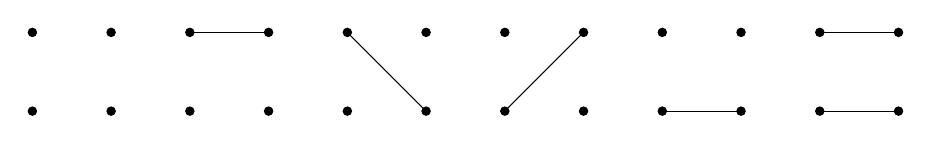
\begin{tikzpicture}
[scale=0.5,x=2cm,y=2cm]
\foreach \x in {0,...,11} \foreach \y in {0,1} \filldraw (\x,\y) circle (3pt); \draw (8,0) -- (9,0); \draw (10,0) -- (11,0);
\draw (10,1) -- (11,1);
\draw (2,1) -- (3,1); \draw (4,1) -- (5,0);\draw (6,0)--(7,1);
\end{tikzpicture}
\caption[Twisted Brandt Monoid]{The twisted Brandt monoid in $P\J_2$}\label{tbc2}
\end{figure}
%\centerline{insert tbc2}
This set forms an involutory subsemigroup of $P\J_2$ with respect to $^\rho$. The mapping that sends each of these
elements in the given order to the matrices given in  (\ref{twisted brandt}) (in the order given there) turns out to be
an isomorphism of involutory semigroups. For the case $n=3$ the same can be done with the members of $P\J_3$ depicted
in Fig.\ \ref{tbc3}.
\begin{figure}[h]
\centering
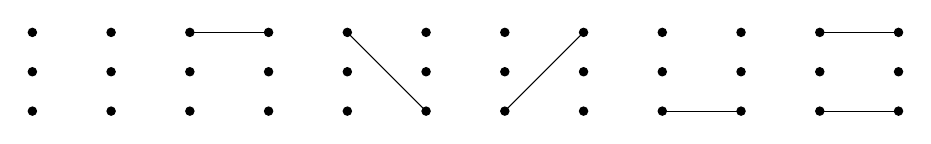
\begin{tikzpicture}
[scale=0.5,x=2cm,y=1cm]
\foreach \x in {0,...,11} \foreach \y in {0,...,2} \filldraw (\x,\y) circle (3pt); \draw (8,0) -- (9,0); \draw (10,0) -- (11,0);
\draw (10,2) -- (11,2);
\draw (2,2) -- (3,2); \draw (4,2) -- (5,0);\draw (6,0)--(7,2);
\end{tikzpicture}
\caption{The twisted Brandt monoid in $P\J_3$}\label{tbc3}
\end{figure}

(2) Since $\J_n\le\A_n\le \B_n$, $\J_n\le\J_{n+2}$ for all $n$ and $\J_n\le \mathfrak{EA}_n$ for all even $n$, by Theorem \ref{TB2} it
suffices to show that $\J_4$ as well as $\J_5$ contains an involutory subsemigroup or divisor isomorphic with the twisted Brandt monoid;
here ``divisor'' means a homomorphic image of an involutory subsemigroup. In the case $n=4$, the same observation as in (1) applies to the
elements of $\J_4$ depicted in Fig.\ \ref{tbj4}.
\begin{figure}[ht]
\centering
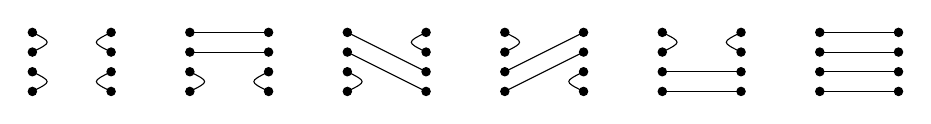
\begin{tikzpicture}
[scale=0.5,x=2cm,y=0.5cm]
\foreach \x in {0,...,11} \foreach \y in {0,...,3} \filldraw (\x,\y) circle (3pt);
\draw (2,3)--(3,3);\draw (2,2)--(3,2);\draw (4,3)--(5,1);\draw (4,2)--(5,0);\draw(6,0)--(7,2);\draw(6,1)--(7,3);\draw(8,0)--(9,0);
\draw(8,1)--(9,1);\foreach \y in {0,...,3} \draw (10,\y)--(11,\y);
\draw (0,0) .. controls (0.25,0.5) and (0.25,0.5).. (0,1);
\draw (0,2) .. controls (0.25,2.5) and (0.25,2.5).. (0,3);
\draw (2,0) .. controls (2.25,0.5) and (2.25,0.5).. (2,1);
\draw (4,0) .. controls (4.25,0.5) and (4.25,0.5).. (4,1);
\draw (6,2) .. controls (6.25,2.5) and (6.25,2.5).. (6,3);
\draw (8,2) .. controls (8.25,2.5) and (8.25,2.5).. (8,3);
\draw (1,0) .. controls (0.75,0.5) and (0.75,0.5).. (1,1);
\draw (1,2) .. controls (0.75,2.5) and (0.75,2.5).. (1,3);
\draw (3,0) .. controls (2.75,0.5) and (2.75,0.5).. (3,1);
\draw (5,2) .. controls (4.75,2.5) and (4.75,2.5).. (5,3);
\draw (7,0) .. controls (6.75,0.5) and (6.75,0.5).. (7,1);
\draw (9,2) .. controls (8.75,2.5) and (8.75,2.5).. (9,3);
\end{tikzpicture}
\caption{The twisted Brandt monoid in $\J_4$}\label{tbj4}
\end{figure}

In case $n=5$ consider the involutory subsemigroup of $\J_5$ generated by the elements of $\J_5$ depicted in Fig.\
\ref{tbj5},
\begin{figure}[h]
\centering
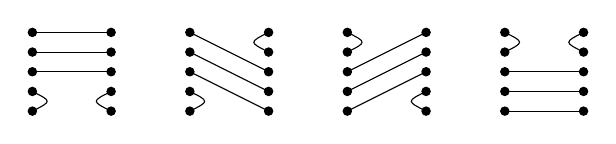
\begin{tikzpicture}
[scale=0.5,x=2cm,y=0.5cm]
\foreach \x in {0,...,7} \foreach \y in {0,...,4} \filldraw (\x,\y) circle (3pt);
\foreach \y in {2,3,4} \draw (0,\y)--(1,\y);
\foreach \y in {2,3,4} \draw (2,\y) -- (3,\y-2);
\foreach \y in {0,1,2} \draw (4,\y)--(5,\y+2);
\foreach \y in {0,1,2} \draw (6,\y)--(7,\y);
\draw (0,0) .. controls (0.25,0.5) and (0.25,0.5).. (0,1);
\draw (2,0) .. controls (2.25,0.5) and (2.25,0.5).. (2,1);
\draw (4,3) .. controls (4.25,3.5) and (4.25,3.5).. (4,4);
\draw (6,3) .. controls (6.25,3.5) and (6.25,3.5).. (6,4);
\draw (1,0) .. controls (0.75,0.5) and (0.75,0.5).. (1,1);
\draw (3,3) .. controls (2.75,3.5) and (2.75,3.5).. (3,4);
\draw (5,0) .. controls (4.75,0.5) and (4.75,0.5).. (5,1);
\draw (7,3) .. controls (6.75,3.5) and (6.75,3.5).. (7,4);
\end{tikzpicture}
\caption{The twisted Brandt monoid in $\var\J_5$}\label{tbj5}
\end{figure}add the identity element of $\J_5$ and factor by the ideal consisting of all elements of rank one. The
result is again an involutory semigroup isomorphic with $\TB$.
\end{proof}

For the remaining cases of small $n$ we note that $P\J_1\cong P\A_1\cong P\B_1\cong \C_1\cong \J_2\cong\mathfrak{EA}_2$ is a two element
semilattice with trivial involution which is finitely based. Moreover, $\J_1\cong \A_1\cong \B_1$ is the trivial involutory semigroup;
$\A_2\cong \B_2$ is a cyclic group of order $2$ with an extra zero element adjoined with trivial involution; $\J_3$ is a $2\times 2$
rectangular band with an extra identity adjoined, the involution satisfying the identity $x=xx^\rho x$---all of these are known to be
finitely based. So we are left with the following two involutory semigroups:

\begin{Problem} Are the involutory semigroups $\A_3$ and $\B_3$ (with respect to $^\rho$) finitely based?
\end{Problem}

\section{Further applications}

\subsection{Unary Rees matrix semigroups}

We had used in \cite{adv} unary Rees matrix semigroups as a tool in the proof of Theorem \ref{Theorem 2.1}; in turn,
here we shall show that this theorem allows one to solve the finite basis problem for a large family of unary Rees
matrix semigroups.

An $I\times I$-matrix $P=(p_{ij})$ over $\mathcal{G}\cup\{0\}$, where $\mathcal{G}$ is a group, is called
\emph{block-diagonalizable} if there exists a partition $\pi$ of the set $I$ such that $p_{ij}\ne 0$ if and only if
$i\m{\pi}j$. If one defines a graph $\Gamma(P)$ on the set $I$ in which two distinct vertices $i$ and $j$ are adjacent
if and only if $p_{ij}\ne0$, then it is clear that block-diagonalizable matrices correspond to graphs whose connected
components are cliques (i.e.\ complete graphs). We say that $P$ is $*$-\emph{regular} if for all $i,j\in I$, one has
$p_{ji}=p_{ij}^{-1}$ whenever $p_{ij}\in \mathcal{G}$ and $p_{ii}=e$, where $e$ is the identity element of
$\mathcal{G}$. (Recall that this property ensures that the unary \Rm\ \sm\ $\Mc^0(I,\mathcal{G},I;P)$ is a regular
$*$-semigroup.)

\begin{Thm}
\label{Rees matrix} Let $P$ be an $I\times I$-matrix over $\mathcal{G}\cup\{0\}$, where $\mathcal{G}$ is a group.
Suppose that $P$ is $*$-regular and not block-diagonalizable. If $\mathcal{G}$ does not belong to the group variety
$\var\mathcal{H}$, where $\mathcal{H}$ is the subgroup generated by the non-zero entries of $P$, then the involutory \Rm\
\sm\ $\Mc^0(I,\mathcal{G},I;P)$ is not finitely based.
\end{Thm}

\begin{proof}
Let $P=(p_{ij})$. Since $P$ is not block-diagonalizable, there is a connected component $C$ in $\Gamma(P)$ which is not a clique. Let $Q$
be a maximal clique in $C$. As $C$ is connected, there exist $i_0\in Q$ and $j_0\in C\setminus Q$ such that $i_0$ and $j_0$ are adjacent.
At the same time, there should be a vertex $k_0\in Q$ such that $j_0$ and $k_0$ are not adjacent---otherwise $Q\cup\{j_0\}$ would make a
larger clique in $C$. Thus, the submatrix $P_0$ of $P$ corresponding to the set $I_0=\{i_0,j_0,k_0\}$ is of the form
$$P_0=\begin{pmatrix}
e      & g & h\\
g^{-1} & e & 0\\
h^{-1} & 0 & e
\end{pmatrix}$$
where $g=p_{i_0j_0},h=p_{i_0k_0}$ belong to $\mathcal{G}$. The unary \Rm\ \sm\ $\Mc^0(I_0,\mathcal{G},I_0;P_0)$ is then
a unary subsemigroup in $\Mc^0(I,\mathcal{G},I;P)$, and the obvious homomorphism $\mathcal{G}\to \mathcal{E}$, where
$\mathcal{E}=\{e\}$ is the trivial group, extends to a unary semigroup homomorphism from
$\Mc^0(I_0,\mathcal{G},I_0;P_0)$ onto $\mathcal{K}_3$. Thus, $\mathcal{K}_3$ belongs to the variety
$\var\Mc^0(I,\mathcal{G},I;P)$.

The Hermitian subsemigroup $\H(\Mc^0(I,\mathcal{G},I;P))$ of $\Mc^0(I,\mathcal{G},I;P)$ is generated by the elements
$(i,e,i)$ where $i$ runs over $I$. This implies that the group coordinates of triples $(i,g,j)$ in
$\H(\Mc^0(I,\mathcal{G},I;P))$ belong to the subgroup $\mathcal{H}$ generated by the non-zero entries of $P$. Hence
$\H(\Mc^0(I,\mathcal{G},I;P))$ is a unary subsemigroup of the unary \Rm\ \sm\ $\Mc^0(I,\mathcal{H},I;P)$. It is not
hard to see that each group in the variety $\var\Mc^0(I,\mathcal{H},I;P)$ belongs to the group variety $\var
\mathcal{H}$. Since $\mathcal{G}$ does not belong to $\var\mathcal{H}$ but obviously belongs to
$\var\Mc^0(I,\mathcal{G},I;P)$, we are in a position to apply Theorem~\ref{Theorem 2.1}.
\end{proof}

A comprehensive treatment of the finite basis problem for unary \Rm\ semigroups forms the subject of a paper by Jackson and the third
author \cite{jacksonvolkov}.

\subsection{Varietal joins}

Recall that the \emph{join} $\mathbf{V}\vee\mathbf{W}$ of two varieties $\mathbf{V}$ and $\mathbf{W}$ is the least
variety containing both $\mathbf{V}$ and $\mathbf{W}$. We show how Theorem~\ref{Theorem 2.1} can be used to produce
interesting examples of non-finitely based joins of varieties of involutory semigroups.

Denote by $\mathbf{CSR^*}$ the variety generated by the regular $^*$-semigroup $\mathcal{K}_3$ (that is, the variety of all
\emph{combinatorial strict regular $*$-semigroups}, see \cite{A1}) and let $\mathbf{I}$ be the variety of all inverse
semigroups.
\begin{Thm}
\label{Theorem 3.2} Let $\pv K$ and $\pv A$ be varieties of involutory semigroups such that:
\begin{enumerate}
\item $\pv K$ contains $\pv{CSR^*}$,
\item $\pv A$ consists of inverse semigroups and contains
a group not contained in $\H(\pv K)$.
\end{enumerate}
Then no variety in the interval $[\pv{CSR^*}\vee \pv A, \pv K\vee\pv{I}]$ is finitely based.
\end{Thm}

\begin{proof}
Let $\mathcal{S}\in \pv K\vee\pv I$; then there exist $\mathcal{K}\in \pv K$, $\mathcal{I}\in \pv I$ such that
$\mathcal{S}$ \emph{divides} (that is, $\mathcal{S}$ is a homomorphic image of a substructure of)
$\mathcal{K}\times\mathcal{I}$ whence $\H(\mathcal{S})$ divides $\H(\mathcal{K})\times \H(\mathcal{I})$. Observe that
$\H(\mathcal{I})$ is a semilattice (with trivial involution). Further, since $\H(\mathcal{K}_3)=\mathcal{K}_3$ and $\pv
{CSR^*}\subseteq \pv K$ we have $\pv{CSR^*}=\H(\pv{CSR^*})\subseteq \H (\pv K)$ so that $\H (\pv K)$ contains all
semilattices with trivial involution since $\pv{CSR^*}$ does so. Altogether, we have $\H(\mathcal{S})\in \H(\pv K)$,
that is $\H(\pv K\vee\pv I)=\H(\pv K)$, and thus, for any variety $\pv V$ in the interval $[\pv{CSR^*}\vee \pv A, \pv
K\vee\pv{I}]$, we have $\H(\pv V)\subseteq \H(\pv K)$. By assumption (2), there exists a group in $\pv A\subseteq \pv
V$ that is not in $\H(\pv K)\supseteq \H(\pv V)$. Thus, Theorem~\ref{Theorem 2.1} applies to the variety~$\pv V$.
\end{proof}

The conditions of Theorem~\ref{Theorem 3.2} are obviously fulfilled if $\pv{CSR^*}\subseteq \pv K$ and $\pv A$ contains a group that is not
in $\pv K$; so, for example $\pv K=[x^m=x^{m+n}]$ for fixed $n\ge 1$ and $m\ge 2$ and $\pv A=\pv G$ (the variety of all groups) meet the
requirements. We mention that Theorem \ref{Theorem 3.2} holds more generally for varieties of \emph{unary} semigroups---it is not really
required that the unary operation in question be an involution.

Recall that a variety $\Vc$ of algebraic structures is a \emph{Cross variety} if
\renewcommand{\labelenumi}{\theenumi)}
\begin{enumerate}
\item $\Vc$ is generated by a finite structure,
\item $\Vc$ contains only finitely many subvarieties,
\item $\Vc$ is finitely based.
\end{enumerate}
For an interesting treatment of Cross varieties of plain semigroups consult Sapir~\cite{S}. The variety $\mathbf{CSR^*}$ is a Cross
variety, see \cite[Theorems 5.1 and 5.2, Corollary 5.4]{A1}. Now let $\mathbf{A}_p$ denote the variety of all abelian groups of exponent
$p$ ($p$ is a prime number); clearly, $\mathbf{A}_p$ is a Cross variety. By \cite[Corollaries 5.4 and 6.5]{A1}, the join
$\mathbf{CSR^*}\vee\mathbf{A}_p$ contains only fourteen subvarieties; however, by the above remark, the join is not finitely based and
therefore is not a Cross variety. We thus have a simple example of two Cross varieties whose join is not a Cross variety. A plain semigroup
example of this kind found in~\cite[Corollary 2.1]{S} is much more involved (with 39 subvarieties).

\section{Existence varieties of locally inverse semigroups}

In this section we give an application to existence varieties of the method of proof of Theorem \ref{Theorem 2.1}.
Recall that an \emph{existence variety} (shortly \emph{e-variety}) of regular semigroups is a class of regular
semigroups closed under taking direct products, \emph{regular} subsemigroups and homomorphic images. This section
assumes the reader's acquaintance with some basics of the theory of regular semigroups.

While research into the structure of regular semigroups was particularly active in the 1970s and early 1980s, a
universal algebra approach for regular semigroups has been introduced at the end of the 1980s by {Ka\softd{}ourek} and
Szendrei \cite{KS} for orthodox semigroups, and, independently, by Hall \cite{H1,H2} for regular semigroups in general.
We shall recall the basic definitions and results necessary to understand the following treatment. For further
information consult the papers \cite{KS,H1,H2,Y1,A2,A3}.

A regular semigroup $\mathcal{S}=\langle S,\cdot\rangle$ is \emph{locally inverse} if for each idempotent $e$ of
$\mathcal S$, the \emph{local submonoid} $eSe$ is an inverse semigroup. The class $L\pv I$ of all (regular) locally
inverse semigroups is a typical example of an existence variety. Observe that \Rm\ semigroups over groups are locally
inverse (moreover, in such a semigroup each local submonoid is a group with 0 adjoined or the trivial group).

It is known \cite[Theorem 7.6]{N1} that a regular semigroup $\mathcal S$ is locally inverse if and only if for any two
$x,y\in \mathcal S$ the set $xV(yx)y$ is a singleton (as usual, $V(z)$ denotes the set of all inverses of the element
$z$). This gives rise to the \emph{sandwich operation} $\wedge$ that can be defined on any locally inverse semigroup by
setting $x\wedge y$ to be the unique element of $xV(yx)y$, so that in this context, locally inverse semigroups are
treated as algebras of type $(2,2)$.

As explained in \cite{A2,A3}, the adequate concept of equational theory for e-varieties of locally inverse semigroups
is based on the signature $\{\cdot,\wedge\}$ and is with respect to a doubled alphabet $X\cup X'$. Here $X$ is, as
usual, a countably infinite set of variables and $X'=\{x'\mid x\in X\}$ is a disjoint copy of $X$; the elements of $X'$
are devoted to represent inverses of the elements which are represented by the elements of $X$. The terms are over this
extended alphabet and are in the signature $\{\cdot,\wedge\}$ where $\cdot$ stands for the associative operation of
multiplication and $\wedge$ for the sandwich operation. Given a term $w(x_1,\dots,x_n,x'_1,\dots,x'_n)$ of this kind, a
value of that term in the locally inverse semigroup $\mathcal S$ is obtained by substituting the variables $x_i,x'_i$
by elements $s_i,s'_i$ in $\mathcal S$ in such a way that each $s'_i$ is an inverse of $s_i$. (In this evaluation it
definitely may happen that distinct variables $x,y$, say, will be substituted with the same element $s$, while the
formal inverses $x'$ and $y'$, respectively, are substituted with distinct inverses $s^\sharp$ and $s^\flat$, say, of
$s$.) Given this notion of evaluation of terms in a locally inverse semigroup, it is clear what it means that a locally
inverse semigroup $\mathcal S$ \emph{satisfies} a \emph{bi-identity} $u=v$ of terms of that kind. The following
Birkhoff type theorem then holds \cite{A2}.

\begin{Thm}\label{Theorem 4.1} A class $\pv V$ of locally inverse semigroups is an
e-variety if and only if it is definable by bi-identities, that is, $\pv V$ consists of all locally inverse semigroups
that satisfy a certain set of bi-identities.\end{Thm}

Now call a set $B$ of bi-identities a \emph{basis} of $\pv V$ if
 a locally inverse semigroup $\mathcal S$ is a member
of $\pv V$ if and only if $\mathcal S$ satisfies all bi-identities of $B$. This semantic notion of basis is equivalent
to a syntactic one: $B$ is a basis of  $\pv V$ if and only if $B$ axiomatizes the \emph{bi-equational theory} which is
the set of all bi-identities over a (fixed) countable infinite set $X$ of variables satisfied by all members of $\pv
V$. The latter means that  each bi-identity satisfied by all members of $\pv V$ can be derived, using natural deduction
rules, from the bi-identities of $B\cup B(L\pv I)$ where $B(L\pv I)$ is a basis for the bi-equational theory of the
class of all locally inverse semigroups. A set consisting of four independent bi-identities which may serve as $B(L\pv
I)$ has been found in \cite{A3}. For more analogues between the theory of e-varieties of regular semigroups and
varieties of universal algebras see \cite{A2,A3,KS,Y1}.

The objective of this section is to obtain an analogue of Theorem~\ref{Theorem 2.1} giving a sufficient condition for
an e-variety $\pv V$ of locally inverse semigroups to have no finite basis of bi-identities.\footnote{The reader may
note that by an argument similar to that in the proof of Proposition 2.9 in \cite{adv} it can be shown that there do
not exist inherently nonfinitely based e-varieties of locally inverse semigroups.} Let $\mathcal S$ be a locally
inverse semigroup and $a_1,\dots,a_k\in \mathcal S$. For each $i$ take an element $a'_i\in V(a_i)$. Then the closure of
the set $\{a_1,\dots,a_k,a'_1,\dots,a'_k\}$ under multiplication and sandwich operation  is a locally inverse
subsemigroup of $\mathcal S$, and is the least locally inverse subsemigroup of $\mathcal S$ containing the set
$\{a_1,\dots,a_k,a'_1,\dots,a'_k\}$ (by \cite{Y1}). We call such a subsemigroup a {\it $k$-generated} locally inverse
subsemigroup of $\mathcal S$. Define the {\it content} $c(t)$ of a term $t$ inductively by $c(x)=c(x')=\{x\}$ and
$c(uv)=c(u\we v)=c(u)\cup c(v)$. In order to prove that an e-variety $\pv V$ has no  finite basis of bi-identities it
is sufficient to prove for each natural number $k$ the existence of a locally inverse semigroup $\mathcal{T}_k$ such
that $\mathcal{T}_k\not\in \pv V$ but $\mathcal{T}_k$ satisfies each bi-identity $u=v$ that holds in $\pv V$ and for
which $\vert c(u)\cup c(v)\vert \le k$. The latter is equivalent to the property that each $k$-generated locally
inverse subsemigroup (as defined above) is contained in~$\pv V$.

For each e-variety $\pv V$ denote by $\Co(\pv V)$ the sub-e-variety of $\pv V$ generated by all idempotent generated
members of $\Vc$. We also need the 5-element \Rm\ semigroup $\mathcal{A}_2$ with the sandwich matrix
\begin{equation}
\label{matrix for TA}
\begin{pmatrix}
0 & e\\
e & e
\end{pmatrix}.
\end{equation} We
are ready to formulate an e-variety analogue of Theorem \ref{Theorem 2.1}.

\begin{Thm}\label{Theorem 4.4} Let $\pv V$ be a locally inverse
e-variety containing the semigroup $\mathcal{A}_2$. If $\pv V$ contains a group which is not in $\Co(\pv V)$ then $\pv
V$ has no finite basis for its bi-identities.
\end{Thm}

\begin{proof} This can be proved in a manner similar to the proof of
Theorem 2.2 in \cite{adv}.  As mentioned above, we have to prove, for each $k$, the existence of a locally inverse
semigroup $\mathcal{T}_k$ such that $\mathcal{T}_k\notin \pv V$ but each $k$-generated locally inverse subsemigroup of
$\mathcal{T}_k$ is contained in $\pv V$.

Let $\mathcal G$ be a group in $\pv V$ that is not contained in $\Co(\pv V)$. Since there must be a bi-identity which
holds in $\Co(\pv V)$ but fails in $\mathcal G$, we may assume that $\mathcal G$ is generated by finitely many
elements, say $g_1,\dots, g_m$, and for convenience we may assume that this set of generators is closed under taking
inverse elements and so generates $\mathcal{G}$ as a semigroup. Next, let $\mathcal{T}_k$ be the \Rm\ semigroup in the
proof of \cite[Theorem 2.2]{adv}, but with $n=2k+1$ being replaced with $n=4k+1$. In that proof it has been shown that
$(1,g_j,mn)\in \left<E(\mathcal{T}_k)\right>$ for $j=1,\dots, m$ (here $\langle E(\mathcal{T}_k)\rangle$ denotes the
idempotent generated subsemigroup of $\mathcal{T}_k$). It follows that $\{1\}\times \mathcal{G}\times\{mn\}\subseteq
\left<E(\mathcal{T}_k)\right>$ whence $\left<E(\mathcal{T}_k)\right>$ contains a subgroup isomorphic to $\mathcal{G}$.
Consequently, $\left<E(\mathcal{T}_k)\right>\notin \Co(\pv V)$ which implies that $\mathcal{T}_k\notin \pv V$.

Finally, consider any $k$-generated locally inverse subsemigroup of $\mathcal{T}_k$, that is, choose elements
$a_1,\dots,a_k,a'_1,\dots,a'_k\in \mathcal{T}_k$ such that $a'_i\in V(a_i)$ for each $i$. Let $\mathcal{T}$ be the
locally inverse subsemigroup generated by $\{a_1,\dots,a_k,a'_1,\dots,a'_k\}$ (that is, the closure of that set under
multiplication and sandwich operation). It is clear that at most $4k$ indices of $\{1,\dots,nm\}$ can occur in the
triple representation of the elements {$a_i$ and $a'_i$}. Therefore, analogously to the unary case proved in
\cite[Theorem 2.2]{adv}, there exist numbers $\la_1,\dots,\la_m$ such that
$$1\le\la_1\le n<\la_2\le 2n < \dots (m-1)n<\la_m\le mn$$
and $\mathcal{T}$ is contained in the semigroup $\mathcal{T}_k(\la_1,\dots,\la_m)$. Again as in Section 1, we can show
that $\mathcal{T}_k(\la_1,\dots,\la_m)$ is isomorphic to a homomorphic image of the direct product $\mathcal{G}\times
\mathcal{U}_k$ of the group $\mathcal G$ and a completely 0-simple semigroup $\mathcal{U}_k$ with trivial subgroups.
Now $\mathcal{G}\in \pv V$ by our assumption and $\mathcal{U}_k\in \pv V$ by a result of Hall \cite{H2} because $\pv V$
contains $\mathcal{A}_2$. This completes the proof.
\end{proof}

Theorem \ref{Theorem 4.4} can be in particular applied to certain joins of e-varieties. Here is an example. Denote by
$\pv{CSR}$ the e-variety generated by the semigroup $\mathcal{A}_2$  and by $\pv {GI}$ the e-variety of all orthodox
locally inverse semigroups (these semigroups are often called \emph{generalized inverse}). The proof of the next
corollary is analogous to that of Theorem~\ref{Theorem 3.2} and is left to the reader.

\begin{Cor} \label{Corollary 4.6} Let $\pv K$ and $\pv A$ be locally inverse
e-varieties such that:
\renewcommand{\labelenumi}{(\theenumi)}
\begin{enumerate}
\item $\pv K$ contains $\pv{CSR}$,
\item $\pv A$ consists of orthodox semigroups and contains a group
not contained in $\Co(\pv K)$.
\end{enumerate}
Then no e-variety in the interval $[\pv{CSR}\vee \pv A, \pv K\vee\pv {GI}]$ is finitely based.
\end{Cor}

\noindent\textbf{Acknowledgements.} The second author was supported by Grant No.\ 174019 of the Ministry of Education and Science of the
Republic of Serbia, and by a grant (Contract 114--451--2002/2011) of the Secretariat of Science and Technological Development of the
Autonomous Province of Vojvodina. The third author acknowledges support from the Russian Foundation for Basic Research, grant 10-01-00524.

\begin{thebibliography}{99}
\frenchspacing

\bibitem{Alm95}
J. Almeida, Finite Semigroups and Universal Algebra, World Scientific, Singapore, 1995.

\bibitem{A1}
K. Auinger, Strict regular $*$-semigroups, in: J. M. Howie, W. D. Munn, H.-J. Weinert (eds.), Proc. Conf. on Semigroups
with Applications, World Scientific, Singapore, 1992, pp. 190--204.

\bibitem{A2}
K. Auinger, The bifree locally inverse semigroup on a set, J. Algebra 166 (1994) 630--650.

\bibitem{A3}
K. Auinger, A system of bi-identities for locally inverse semigroups, Proc. Amer. Math. Soc. 123 (1995) 979--988.

\bibitem{pseudovarieties}
K. Auinger, Pseudovarieties generated by Brauer-type monoids, Forum Math. (to appear), \url{http://dx.doi.org/10.1515/form.2011.146}.

\bibitem{complexity}
K. Auinger, Krohn--Rhodes complexity of Brauer-type semigroups, preprint,
\url{http://arxiv.org/pdf/1202.4982.pdf}.

\bibitem{adv}
K. Auinger, I. Dolinka, M. V. Volkov, Matrix identities involving multiplication and transposition, J. Eur. Math. Soc. 14 (2012) 937--969.

\bibitem{brauer}
R. Brauer, On algebras which are connected with the semisimple continuous groups, Ann. Math. 38 (1937) 857--872.

\bibitem{BuSa81}
S. Burris, H. P. Sankappanavar, A Course in Universal Algebra, Springer-Verlag, Berlin--Heidelberg--New York, 1981.

\bibitem{CP}
A. H. Clifford, G. B. Preston, The Algebraic Theory of Semigroups, Vol. I, Amer. Math. Soc., Providence, 1961.

\bibitem{grahamlehrer}
J. J. Graham, G. I. Lehrer, Cellular algebras, Invent. Math. 123 (1996) 1--34.

\bibitem{H1}
T. E. Hall, Identities for existence varieties of regular semigroups, Bull. Austral. Math. Soc. 40 (1989) 59--77.

\bibitem{H2}
T. E. Hall, Regular semigroups: amalgamation and the lattice of existence varieties, Algebra Univers. 29 (1991)
79--108.

\bibitem{jacksonvolkov}
M. Jackson, M. V. Volkov, The algebra of adjacency patterns: Rees matrix semigroups with reversion, in: A. Blass, N. Dershowitz, W. Reisig
(eds.), Fields of Logic and Computation, Essays Dedicated to Yuri Gurevich on the Occasion of His 70th Birthday, Lect. Notes Comp. Sci.
Vol. 6300, Springer-Verlag, Berlin--Heidelberg--New York, 2010, pp. 414--443.

\bibitem{jones}
V. F. R. Jones, A quotient of the affine Hecke algebra in the Brauer algebra, Enseign. Math. II. S\'er. 40 (1994)
313--344.

\bibitem{KS}
J. {Ka\softd{}ourek}, M. B. Szendrei, A new approach in the theory of orthodox semigroups, Semigroup Forum 40 (1990)
257--296.

\bibitem{KR}
K. H. Kim, F. Roush, On groups in varieties of semigroups, Semigroup Forum 16 (1978) 201--202.

\bibitem{Kru}
R. L. Kruse, Identities satisfied by a finite ring, J. Algebra 26 (1973) 298--318.

\bibitem{KMM}
G. Kudryavtseva, V. Maltcev, V. Mazorchuk, ${\mathcal L}$- and $\mathcal R$-cross-sections in the Brauer semigroup,
Semigroup Forum 72 (2006) 223--248.

\bibitem{KM2}
G. Kudryavtseva, V. Mazorchuk, On presentations of Brauer-type monoids, Central Eur. J. Math. 4 (2006) 413--434.

\bibitem{fitzgerald}
K. W. Lau, D. G. Fitzgerald, Ideal structure of the Kauffman and related monoids, Comm. Algebra 34 (2006) 2617--2629.

\bibitem{Lvov}
I. V. L'vov, Varieties of associative rings. I, II, Algebra i Logika 12 (1973) 269--297, 363; ibid. 667--688, 735
(Russian).

\bibitem{malcevmazorchuk}
V. Maltcev, V. Mazorchuk, Presentation of the singular part of the Brauer monoid, Math. Bohem. 132 (2007) 297--323.

\bibitem{martin}
P. Martin, The structure of partition algebras, J. Algebra 183 (1996) 319--358.

\bibitem{Maz1}
V. Mazorchuk, On the structure of Brauer semigroups and its partial analogue, Problems in Algebra 13 (1998) 29--45.

\bibitem{Maz2}
V. Mazorchuk, Endomorphisms of $\B_n$, ${\mathcal P}\B_n$ and $\C_n$, Comm. Algebra 30 (2002) 3489--3513.

\bibitem{McK1}
R. McKenzie, Equational bases for lattice theories,  Math. Scand. 27 (1970) 24--38.

\bibitem{McK2}
R. McKenzie, A new product of algebras and a type reduction theorem, Algebra Univers. 18 (1984), 29--69.

\bibitem{McK3}
R. McKenzie, Tarski's finite basis problem is undecidable, Internat. J. Algebra Comput. 6 (1996) 49--104.

\bibitem{McNSh}
G. McNulty, C. Shallon, Inherently nonfinitely based finite algebras, in: R. S. Freese, O. C. Garc\'{\i}a (eds.), Universal Algebra and
Lattice Theory (Puebla, 1982), Lect. Notes Math. Vol. 1004, Springer-Verlag, Berlin--Heidelberg--New York, 1983, pp. 206--231

\bibitem{N1}
K. S. S. Nambooripad, Structure of regular semigroups. I, Mem. Amer. Math. Soc. 22 (1979), no. 224, vii+119 pp.

\bibitem{N2}
K. S. S. Nambooripad, The natural partial order on a regular semigroup, Proc. Edinburgh Math. Soc. 32 (1980) 249--260.

\bibitem{Ne}
H. Neumann, Varieties of Groups, Springer-Verlag, Berlin--Heidelberg--New York, 1967.

\bibitem{OP}
S. Oates, M. B. Powell, Identical relations in finite groups, J. Algebra 1 (1964) 11--39.

\bibitem{Per69}
P. Perkins, Bases for equational theories of semigroups, J. Algebra 11 (1969) 298--314.

\bibitem{Per89}
P. Perkins, Finite axiomatizability for equational theories of computable groupoids, J. Symbolic Logic 54 (1989)
1018--1022.

\bibitem{S}
M. V. Sapir, On Cross semigroup varieties and related questions, Semigroup Forum 42 (1991) 345--364.

\bibitem{temperleylieb}
H. N. V. Temperley, E. H. Lieb, Relations between the `percolation' and `coloring' problem and other graph-theoretic
problems associated with regular planar lattices: some exact results for the `percolation' problem, Proc. Roy. Soc.
London Ser.~A  322 (1971) 251--280.

\bibitem{volkovjaponicae}
M. V. Volkov, The finite basis problem for finite semigroups, Sci. Math. Jpn. 53 (2001) 171--199.

\bibitem{Wil}
S. Wilcox, Cellularity of diagram algebras as twisted semigroup algebras, J. Algebra 309 (2007), 10--31.

\bibitem{xi}
C. Xi, Partition algebras are cellular, Comp. Math. 119 (1999) 99--109.

\bibitem{Y1}
Y. T. Yeh, The existence of $e$-free objects in {$e$-varieties} of regular semigroups, Internat. J. Algebra Comput. 2
(1992) 471--484.
\end{thebibliography}

\end{document}
